\documentclass[twoside]{book}

% Packages required by doxygen
\usepackage{fixltx2e}
\usepackage{calc}
\usepackage{doxygen}
\usepackage[export]{adjustbox} % also loads graphicx
\usepackage{graphicx}
\usepackage[utf8]{inputenc}
\usepackage{makeidx}
\usepackage{multicol}
\usepackage{multirow}
\PassOptionsToPackage{warn}{textcomp}
\usepackage{textcomp}
\usepackage[nointegrals]{wasysym}
\usepackage[table]{xcolor}

% Font selection
\usepackage[T1]{fontenc}
\usepackage[scaled=.90]{helvet}
\usepackage{courier}
\usepackage{amssymb}
\usepackage{sectsty}
\renewcommand{\familydefault}{\sfdefault}
\allsectionsfont{%
  \fontseries{bc}\selectfont%
  \color{darkgray}%
}
\renewcommand{\DoxyLabelFont}{%
  \fontseries{bc}\selectfont%
  \color{darkgray}%
}
\newcommand{\+}{\discretionary{\mbox{\scriptsize$\hookleftarrow$}}{}{}}

% Page & text layout
\usepackage{geometry}
\geometry{%
  a4paper,%
  top=2.5cm,%
  bottom=2.5cm,%
  left=2.5cm,%
  right=2.5cm%
}
\tolerance=750
\hfuzz=15pt
\hbadness=750
\setlength{\emergencystretch}{15pt}
\setlength{\parindent}{0cm}
\setlength{\parskip}{3ex plus 2ex minus 2ex}
\makeatletter
\renewcommand{\paragraph}{%
  \@startsection{paragraph}{4}{0ex}{-1.0ex}{1.0ex}{%
    \normalfont\normalsize\bfseries\SS@parafont%
  }%
}
\renewcommand{\subparagraph}{%
  \@startsection{subparagraph}{5}{0ex}{-1.0ex}{1.0ex}{%
    \normalfont\normalsize\bfseries\SS@subparafont%
  }%
}
\makeatother

% Headers & footers
\usepackage{fancyhdr}
\pagestyle{fancyplain}
\fancyhead[LE]{\fancyplain{}{\bfseries\thepage}}
\fancyhead[CE]{\fancyplain{}{}}
\fancyhead[RE]{\fancyplain{}{\bfseries\leftmark}}
\fancyhead[LO]{\fancyplain{}{\bfseries\rightmark}}
\fancyhead[CO]{\fancyplain{}{}}
\fancyhead[RO]{\fancyplain{}{\bfseries\thepage}}
\fancyfoot[LE]{\fancyplain{}{}}
\fancyfoot[CE]{\fancyplain{}{}}
\fancyfoot[RE]{\fancyplain{}{\bfseries\scriptsize Generated by Doxygen }}
\fancyfoot[LO]{\fancyplain{}{\bfseries\scriptsize Generated by Doxygen }}
\fancyfoot[CO]{\fancyplain{}{}}
\fancyfoot[RO]{\fancyplain{}{}}
\renewcommand{\footrulewidth}{0.4pt}
\renewcommand{\chaptermark}[1]{%
  \markboth{#1}{}%
}
\renewcommand{\sectionmark}[1]{%
  \markright{\thesection\ #1}%
}

% Indices & bibliography
\usepackage{natbib}
\usepackage[titles]{tocloft}
\setcounter{tocdepth}{3}
\setcounter{secnumdepth}{5}
\makeindex

% Hyperlinks (required, but should be loaded last)
\usepackage{ifpdf}
\ifpdf
  \usepackage[pdftex,pagebackref=true]{hyperref}
\else
  \usepackage[ps2pdf,pagebackref=true]{hyperref}
\fi
\hypersetup{%
  colorlinks=true,%
  linkcolor=blue,%
  citecolor=blue,%
  unicode%
}

% Custom commands
\newcommand{\clearemptydoublepage}{%
  \newpage{\pagestyle{empty}\cleardoublepage}%
}

\usepackage{caption}
\captionsetup{labelsep=space,justification=centering,font={bf},singlelinecheck=off,skip=4pt,position=top}

%===== C O N T E N T S =====

\begin{document}

% Titlepage & ToC
\hypersetup{pageanchor=false,
             bookmarksnumbered=true,
             pdfencoding=unicode
            }
\pagenumbering{alph}
\begin{titlepage}
\vspace*{7cm}
\begin{center}%
{\Large Spaceship Rescue }\\
\vspace*{1cm}
{\large Generated by Doxygen 1.8.14}\\
\end{center}
\end{titlepage}
\clearemptydoublepage
\pagenumbering{roman}
\tableofcontents
\clearemptydoublepage
\pagenumbering{arabic}
\hypersetup{pageanchor=true}

%--- Begin generated contents ---
\chapter{Hierarchical Index}
\section{Class Hierarchy}
This inheritance list is sorted roughly, but not completely, alphabetically\+:\begin{DoxyCompactList}
\item \contentsline{section}{Animation}{\pageref{class_animation}}{}
\item \contentsline{section}{Arc}{\pageref{class_arc}}{}
\item \contentsline{section}{A\+Star}{\pageref{class_a_star}}{}
\item Drawable\begin{DoxyCompactList}
\item \contentsline{section}{Animated\+Sprite}{\pageref{class_animated_sprite}}{}
\end{DoxyCompactList}
\item \contentsline{section}{Nest}{\pageref{class_nest}}{}
\item \contentsline{section}{Node}{\pageref{class_node}}{}
\item \contentsline{section}{Node\+Layout}{\pageref{class_node_layout}}{}
\item \contentsline{section}{Node\+Search\+Cost\+Comparer\+A\+Star}{\pageref{class_node_search_cost_comparer_a_star}}{}
\item \contentsline{section}{Node\+Search\+Cost\+Comparer\+U\+CS}{\pageref{class_node_search_cost_comparer_u_c_s}}{}
\item \contentsline{section}{Player}{\pageref{class_player}}{}
\item \contentsline{section}{Power\+Up}{\pageref{class_power_up}}{}
\begin{DoxyCompactList}
\item \contentsline{section}{Fire\+Rate\+Power\+Up}{\pageref{class_fire_rate_power_up}}{}
\item \contentsline{section}{Health\+Power\+Up}{\pageref{class_health_power_up}}{}
\item \contentsline{section}{Shield\+Power\+Up}{\pageref{class_shield_power_up}}{}
\end{DoxyCompactList}
\item \contentsline{section}{Predator\+Ship}{\pageref{class_predator_ship}}{}
\item \contentsline{section}{Projectile}{\pageref{class_projectile}}{}
\item \contentsline{section}{Seeker\+Missile}{\pageref{class_seeker_missile}}{}
\item \contentsline{section}{Space\+Station}{\pageref{class_space_station}}{}
\item \contentsline{section}{Sweeper\+Boid}{\pageref{class_sweeper_boid}}{}
\item \contentsline{section}{Tile}{\pageref{class_tile}}{}
\begin{DoxyCompactList}
\item \contentsline{section}{Floor}{\pageref{class_floor}}{}
\item \contentsline{section}{Wall}{\pageref{class_wall}}{}
\end{DoxyCompactList}
\item Transformable\begin{DoxyCompactList}
\item \contentsline{section}{Animated\+Sprite}{\pageref{class_animated_sprite}}{}
\end{DoxyCompactList}
\item \contentsline{section}{Worker}{\pageref{class_worker}}{}
\item \contentsline{section}{World}{\pageref{class_world}}{}
\end{DoxyCompactList}

\chapter{Class Index}
\section{Class List}
Here are the classes, structs, unions and interfaces with brief descriptions\+:\begin{DoxyCompactList}
\item\contentsline{section}{\mbox{\hyperlink{class_animated_sprite}{Animated\+Sprite}} }{\pageref{class_animated_sprite}}{}
\item\contentsline{section}{\mbox{\hyperlink{class_animation}{Animation}} }{\pageref{class_animation}}{}
\item\contentsline{section}{\mbox{\hyperlink{class_arc}{Arc}} }{\pageref{class_arc}}{}
\item\contentsline{section}{\mbox{\hyperlink{class_a_star}{A\+Star}} }{\pageref{class_a_star}}{}
\item\contentsline{section}{\mbox{\hyperlink{class_fire_rate_power_up}{Fire\+Rate\+Power\+Up}} }{\pageref{class_fire_rate_power_up}}{}
\item\contentsline{section}{\mbox{\hyperlink{class_floor}{Floor}} }{\pageref{class_floor}}{}
\item\contentsline{section}{\mbox{\hyperlink{class_health_power_up}{Health\+Power\+Up}} }{\pageref{class_health_power_up}}{}
\item\contentsline{section}{\mbox{\hyperlink{class_nest}{Nest}} }{\pageref{class_nest}}{}
\item\contentsline{section}{\mbox{\hyperlink{class_node}{Node}} }{\pageref{class_node}}{}
\item\contentsline{section}{\mbox{\hyperlink{class_node_layout}{Node\+Layout}} }{\pageref{class_node_layout}}{}
\item\contentsline{section}{\mbox{\hyperlink{class_node_search_cost_comparer_a_star}{Node\+Search\+Cost\+Comparer\+A\+Star}} }{\pageref{class_node_search_cost_comparer_a_star}}{}
\item\contentsline{section}{\mbox{\hyperlink{class_node_search_cost_comparer_u_c_s}{Node\+Search\+Cost\+Comparer\+U\+CS}} }{\pageref{class_node_search_cost_comparer_u_c_s}}{}
\item\contentsline{section}{\mbox{\hyperlink{class_player}{Player}} }{\pageref{class_player}}{}
\item\contentsline{section}{\mbox{\hyperlink{class_power_up}{Power\+Up}} }{\pageref{class_power_up}}{}
\item\contentsline{section}{\mbox{\hyperlink{class_predator_ship}{Predator\+Ship}} }{\pageref{class_predator_ship}}{}
\item\contentsline{section}{\mbox{\hyperlink{class_projectile}{Projectile}} }{\pageref{class_projectile}}{}
\item\contentsline{section}{\mbox{\hyperlink{class_seeker_missile}{Seeker\+Missile}} }{\pageref{class_seeker_missile}}{}
\item\contentsline{section}{\mbox{\hyperlink{class_shield_power_up}{Shield\+Power\+Up}} }{\pageref{class_shield_power_up}}{}
\item\contentsline{section}{\mbox{\hyperlink{class_space_station}{Space\+Station}} }{\pageref{class_space_station}}{}
\item\contentsline{section}{\mbox{\hyperlink{class_sweeper_boid}{Sweeper\+Boid}} }{\pageref{class_sweeper_boid}}{}
\item\contentsline{section}{\mbox{\hyperlink{class_tile}{Tile}} }{\pageref{class_tile}}{}
\item\contentsline{section}{\mbox{\hyperlink{class_wall}{Wall}} }{\pageref{class_wall}}{}
\item\contentsline{section}{\mbox{\hyperlink{class_worker}{Worker}} }{\pageref{class_worker}}{}
\item\contentsline{section}{\mbox{\hyperlink{class_world}{World}} }{\pageref{class_world}}{}
\end{DoxyCompactList}

\chapter{Class Documentation}
\hypertarget{class_animated_sprite}{}\section{Animated\+Sprite Class Reference}
\label{class_animated_sprite}\index{Animated\+Sprite@{Animated\+Sprite}}
Inheritance diagram for Animated\+Sprite\+:\begin{figure}[H]
\begin{center}
\leavevmode
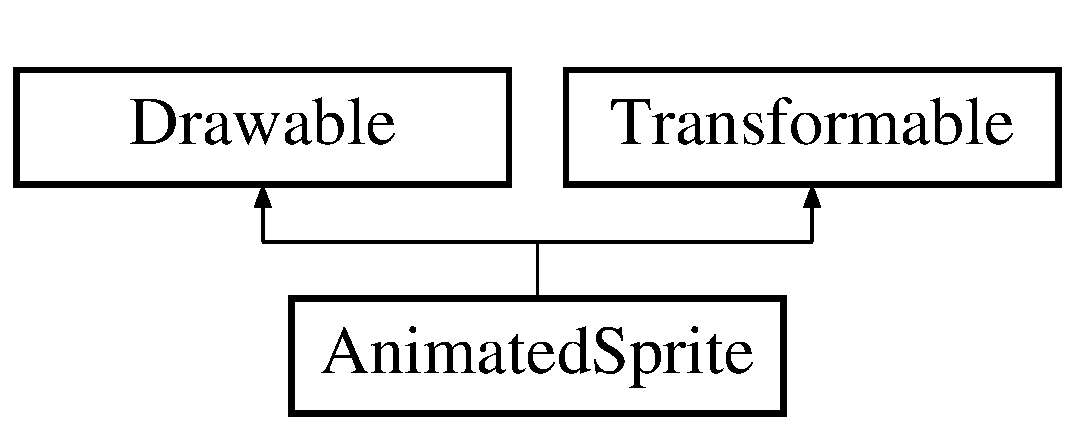
\includegraphics[height=2.000000cm]{class_animated_sprite}
\end{center}
\end{figure}
\subsection*{Public Member Functions}
\begin{DoxyCompactItemize}
\item 
\mbox{\Hypertarget{class_animated_sprite_a097ab8444824e7085d71a1f7144e7763}\label{class_animated_sprite_a097ab8444824e7085d71a1f7144e7763}} 
{\bfseries Animated\+Sprite} (sf\+::\+Time frame\+Time=sf\+::seconds(0.\+2f), bool paused=false, bool looped=true)
\item 
\mbox{\Hypertarget{class_animated_sprite_a17a41ff812631a9d8947d272933d6696}\label{class_animated_sprite_a17a41ff812631a9d8947d272933d6696}} 
void {\bfseries update} (sf\+::\+Time delta\+Time)
\item 
\mbox{\Hypertarget{class_animated_sprite_ab1afc57d90d57a0c4bc4f5b090f2dacf}\label{class_animated_sprite_ab1afc57d90d57a0c4bc4f5b090f2dacf}} 
void {\bfseries set\+Animation} (const \mbox{\hyperlink{class_animation}{Animation}} \&animation)
\item 
\mbox{\Hypertarget{class_animated_sprite_af598fab5c3599ccc5ed1e2d4fefa68cc}\label{class_animated_sprite_af598fab5c3599ccc5ed1e2d4fefa68cc}} 
void {\bfseries set\+Frame\+Time} (sf\+::\+Time time)
\item 
\mbox{\Hypertarget{class_animated_sprite_a203b968f1cb374cca5dbc89716174020}\label{class_animated_sprite_a203b968f1cb374cca5dbc89716174020}} 
void {\bfseries play} ()
\item 
\mbox{\Hypertarget{class_animated_sprite_a9ea345649a4e012d096bc04aafe1ecb0}\label{class_animated_sprite_a9ea345649a4e012d096bc04aafe1ecb0}} 
void {\bfseries play} (const \mbox{\hyperlink{class_animation}{Animation}} \&animation)
\item 
\mbox{\Hypertarget{class_animated_sprite_a48384db59427423b5c1d98f6ee94fe45}\label{class_animated_sprite_a48384db59427423b5c1d98f6ee94fe45}} 
void {\bfseries pause} ()
\item 
\mbox{\Hypertarget{class_animated_sprite_af9734f4346d3d2370322b2dcaeef133c}\label{class_animated_sprite_af9734f4346d3d2370322b2dcaeef133c}} 
void {\bfseries stop} ()
\item 
\mbox{\Hypertarget{class_animated_sprite_a855a5a48ea2e1c51c7c9304857dd2f8c}\label{class_animated_sprite_a855a5a48ea2e1c51c7c9304857dd2f8c}} 
void {\bfseries set\+Looped} (bool looped)
\item 
\mbox{\Hypertarget{class_animated_sprite_a1a96a0f6570efddd2eb26f89bc5b6f50}\label{class_animated_sprite_a1a96a0f6570efddd2eb26f89bc5b6f50}} 
void {\bfseries set\+Color} (const sf\+::\+Color \&color)
\item 
\mbox{\Hypertarget{class_animated_sprite_a03bacdbaf638cb6f7987e342980206c2}\label{class_animated_sprite_a03bacdbaf638cb6f7987e342980206c2}} 
const \mbox{\hyperlink{class_animation}{Animation}} $\ast$ {\bfseries get\+Animation} () const
\item 
\mbox{\Hypertarget{class_animated_sprite_ac4c88435c8698f452629c5cd78bfb3c9}\label{class_animated_sprite_ac4c88435c8698f452629c5cd78bfb3c9}} 
sf\+::\+Float\+Rect {\bfseries get\+Local\+Bounds} () const
\item 
\mbox{\Hypertarget{class_animated_sprite_a86dca0906c53b3e630aaeac2f0085a0e}\label{class_animated_sprite_a86dca0906c53b3e630aaeac2f0085a0e}} 
sf\+::\+Float\+Rect {\bfseries get\+Global\+Bounds} () const
\item 
\mbox{\Hypertarget{class_animated_sprite_aaf2c2fb0e1487e689af4a6bbeb7e3e85}\label{class_animated_sprite_aaf2c2fb0e1487e689af4a6bbeb7e3e85}} 
bool {\bfseries is\+Looped} () const
\item 
\mbox{\Hypertarget{class_animated_sprite_a55f450add05d45e5369a6ad24f9e438f}\label{class_animated_sprite_a55f450add05d45e5369a6ad24f9e438f}} 
bool {\bfseries is\+Playing} () const
\item 
\mbox{\Hypertarget{class_animated_sprite_a5291f8e24fe2c6e4284bc7ff9499ef77}\label{class_animated_sprite_a5291f8e24fe2c6e4284bc7ff9499ef77}} 
sf\+::\+Time {\bfseries get\+Frame\+Time} () const
\item 
\mbox{\Hypertarget{class_animated_sprite_a0b3e38fffdc1d29f46fa08df9ef2a747}\label{class_animated_sprite_a0b3e38fffdc1d29f46fa08df9ef2a747}} 
void {\bfseries set\+Frame} (std\+::size\+\_\+t new\+Frame, bool reset\+Time=true)
\end{DoxyCompactItemize}


The documentation for this class was generated from the following files\+:\begin{DoxyCompactItemize}
\item 
Animated\+Sprite.\+hpp\item 
Animated\+Sprite.\+cpp\end{DoxyCompactItemize}

\hypertarget{class_animation}{}\section{Animation Class Reference}
\label{class_animation}\index{Animation@{Animation}}
\subsection*{Public Member Functions}
\begin{DoxyCompactItemize}
\item 
\mbox{\Hypertarget{class_animation_a486ee5fa2d40ae90f227a19866998c91}\label{class_animation_a486ee5fa2d40ae90f227a19866998c91}} 
void {\bfseries add\+Frame} (sf\+::\+Int\+Rect rect)
\item 
\mbox{\Hypertarget{class_animation_a2fb16f452a323d51a0104c0aa454cab3}\label{class_animation_a2fb16f452a323d51a0104c0aa454cab3}} 
void {\bfseries set\+Sprite\+Sheet} (const sf\+::\+Texture \&texture)
\item 
\mbox{\Hypertarget{class_animation_abf4f00f8b1657829583d7d92e71b93d1}\label{class_animation_abf4f00f8b1657829583d7d92e71b93d1}} 
const sf\+::\+Texture $\ast$ {\bfseries get\+Sprite\+Sheet} () const
\item 
\mbox{\Hypertarget{class_animation_ac6854dc96e9fc8ffd97feba43547c869}\label{class_animation_ac6854dc96e9fc8ffd97feba43547c869}} 
std\+::size\+\_\+t {\bfseries get\+Size} () const
\item 
\mbox{\Hypertarget{class_animation_a8cf30a3b19ba104eeb34b08f45cfabe2}\label{class_animation_a8cf30a3b19ba104eeb34b08f45cfabe2}} 
const sf\+::\+Int\+Rect \& {\bfseries get\+Frame} (std\+::size\+\_\+t n) const
\end{DoxyCompactItemize}


The documentation for this class was generated from the following files\+:\begin{DoxyCompactItemize}
\item 
Animation.\+hpp\item 
Animation.\+cpp\end{DoxyCompactItemize}

\hypertarget{class_arc}{}\section{Arc Class Reference}
\label{class_arc}\index{Arc@{Arc}}
\subsection*{Public Member Functions}
\begin{DoxyCompactItemize}
\item 
\mbox{\Hypertarget{class_arc_afe60276bd76872e03a6cabf5f7af6474}\label{class_arc_afe60276bd76872e03a6cabf5f7af6474}} 
void {\bfseries set\+Node} (\mbox{\hyperlink{class_node}{Node}} $\ast$n)
\item 
\mbox{\Hypertarget{class_arc_a26c9cc309b27a33a64cb3da129aa548c}\label{class_arc_a26c9cc309b27a33a64cb3da129aa548c}} 
\mbox{\hyperlink{class_node}{Node}} $\ast$ {\bfseries get\+Node} ()
\item 
\mbox{\Hypertarget{class_arc_a9339b212a1c053b0fec4a56326104b82}\label{class_arc_a9339b212a1c053b0fec4a56326104b82}} 
void {\bfseries set\+Weight} (float w)
\item 
\mbox{\Hypertarget{class_arc_a2b914759c552c7a732c2fdabe1dd3393}\label{class_arc_a2b914759c552c7a732c2fdabe1dd3393}} 
float {\bfseries get\+Weight} ()
\end{DoxyCompactItemize}


The documentation for this class was generated from the following files\+:\begin{DoxyCompactItemize}
\item 
Arc.\+h\item 
Arc.\+cpp\end{DoxyCompactItemize}

\hypertarget{class_a_star}{}\section{A\+Star Class Reference}
\label{class_a_star}\index{A\+Star@{A\+Star}}
\subsection*{Public Member Functions}
\begin{DoxyCompactItemize}
\item 
\mbox{\Hypertarget{class_a_star_ab0b03d0729eb5cbf94969544dfaf8802}\label{class_a_star_ab0b03d0729eb5cbf94969544dfaf8802}} 
{\bfseries A\+Star} (\mbox{\hyperlink{class_node_layout}{Node\+Layout}} \&nodes)
\item 
\mbox{\Hypertarget{class_a_star_af4b37efdae8b35ee5a07c955a50ed192}\label{class_a_star_af4b37efdae8b35ee5a07c955a50ed192}} 
void {\bfseries calculate\+Path} (\mbox{\hyperlink{class_node}{Node}} $\ast$p\+Start, \mbox{\hyperlink{class_node}{Node}} $\ast$p\+Dest, std\+::vector$<$ \mbox{\hyperlink{class_node}{Node}} $\ast$$>$ \&path)
\end{DoxyCompactItemize}


The documentation for this class was generated from the following files\+:\begin{DoxyCompactItemize}
\item 
A\+Star.\+h\item 
A\+Star.\+cpp\end{DoxyCompactItemize}

\hypertarget{class_fire_rate_power_up}{}\section{Fire\+Rate\+Power\+Up Class Reference}
\label{class_fire_rate_power_up}\index{Fire\+Rate\+Power\+Up@{Fire\+Rate\+Power\+Up}}
Inheritance diagram for Fire\+Rate\+Power\+Up\+:\begin{figure}[H]
\begin{center}
\leavevmode
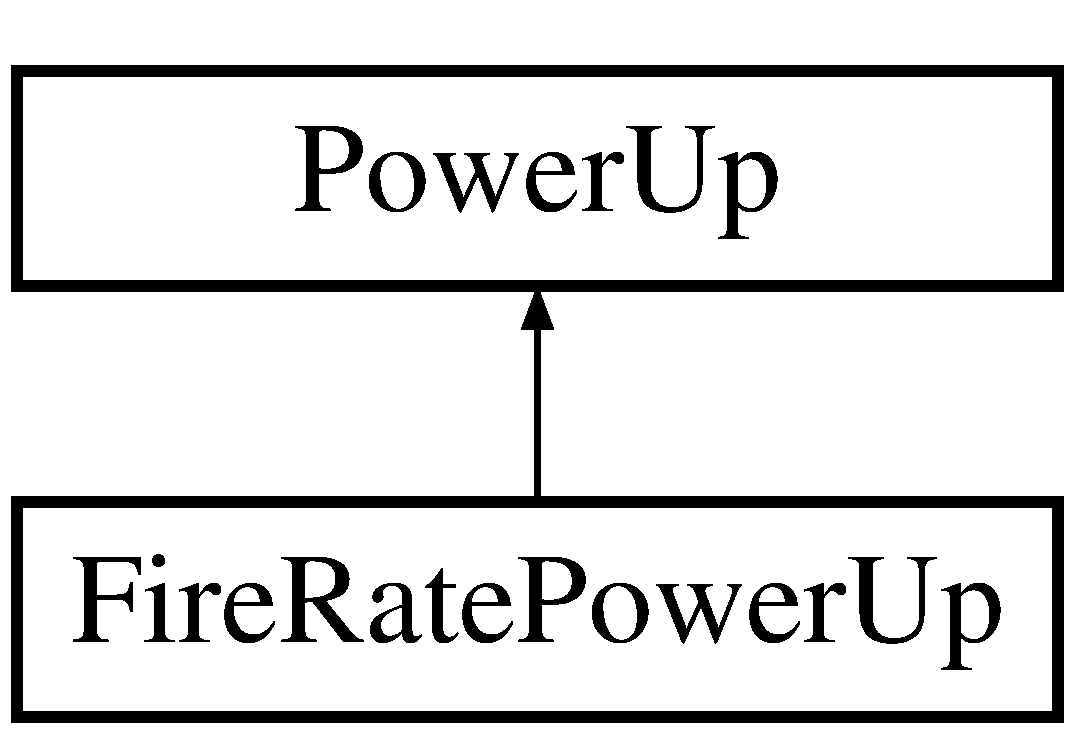
\includegraphics[height=2.000000cm]{class_fire_rate_power_up}
\end{center}
\end{figure}
\subsection*{Public Member Functions}
\begin{DoxyCompactItemize}
\item 
\mbox{\Hypertarget{class_fire_rate_power_up_a70d9addd3e9d0d7ad3d4a26f0ae65bc9}\label{class_fire_rate_power_up_a70d9addd3e9d0d7ad3d4a26f0ae65bc9}} 
{\bfseries Fire\+Rate\+Power\+Up} (sf\+::\+Vector2f pos)
\item 
\mbox{\Hypertarget{class_fire_rate_power_up_a728e0416b3523ba8922ac0880887d327}\label{class_fire_rate_power_up_a728e0416b3523ba8922ac0880887d327}} 
void {\bfseries check\+Collision} (\mbox{\hyperlink{class_player}{Player}} $\ast$player)
\end{DoxyCompactItemize}
\subsection*{Additional Inherited Members}


The documentation for this class was generated from the following files\+:\begin{DoxyCompactItemize}
\item 
Fire\+Rate\+Power\+Up.\+h\item 
Fire\+Rate\+Power\+Up.\+cpp\end{DoxyCompactItemize}

\hypertarget{class_floor}{}\section{Floor Class Reference}
\label{class_floor}\index{Floor@{Floor}}
Inheritance diagram for Floor\+:\begin{figure}[H]
\begin{center}
\leavevmode
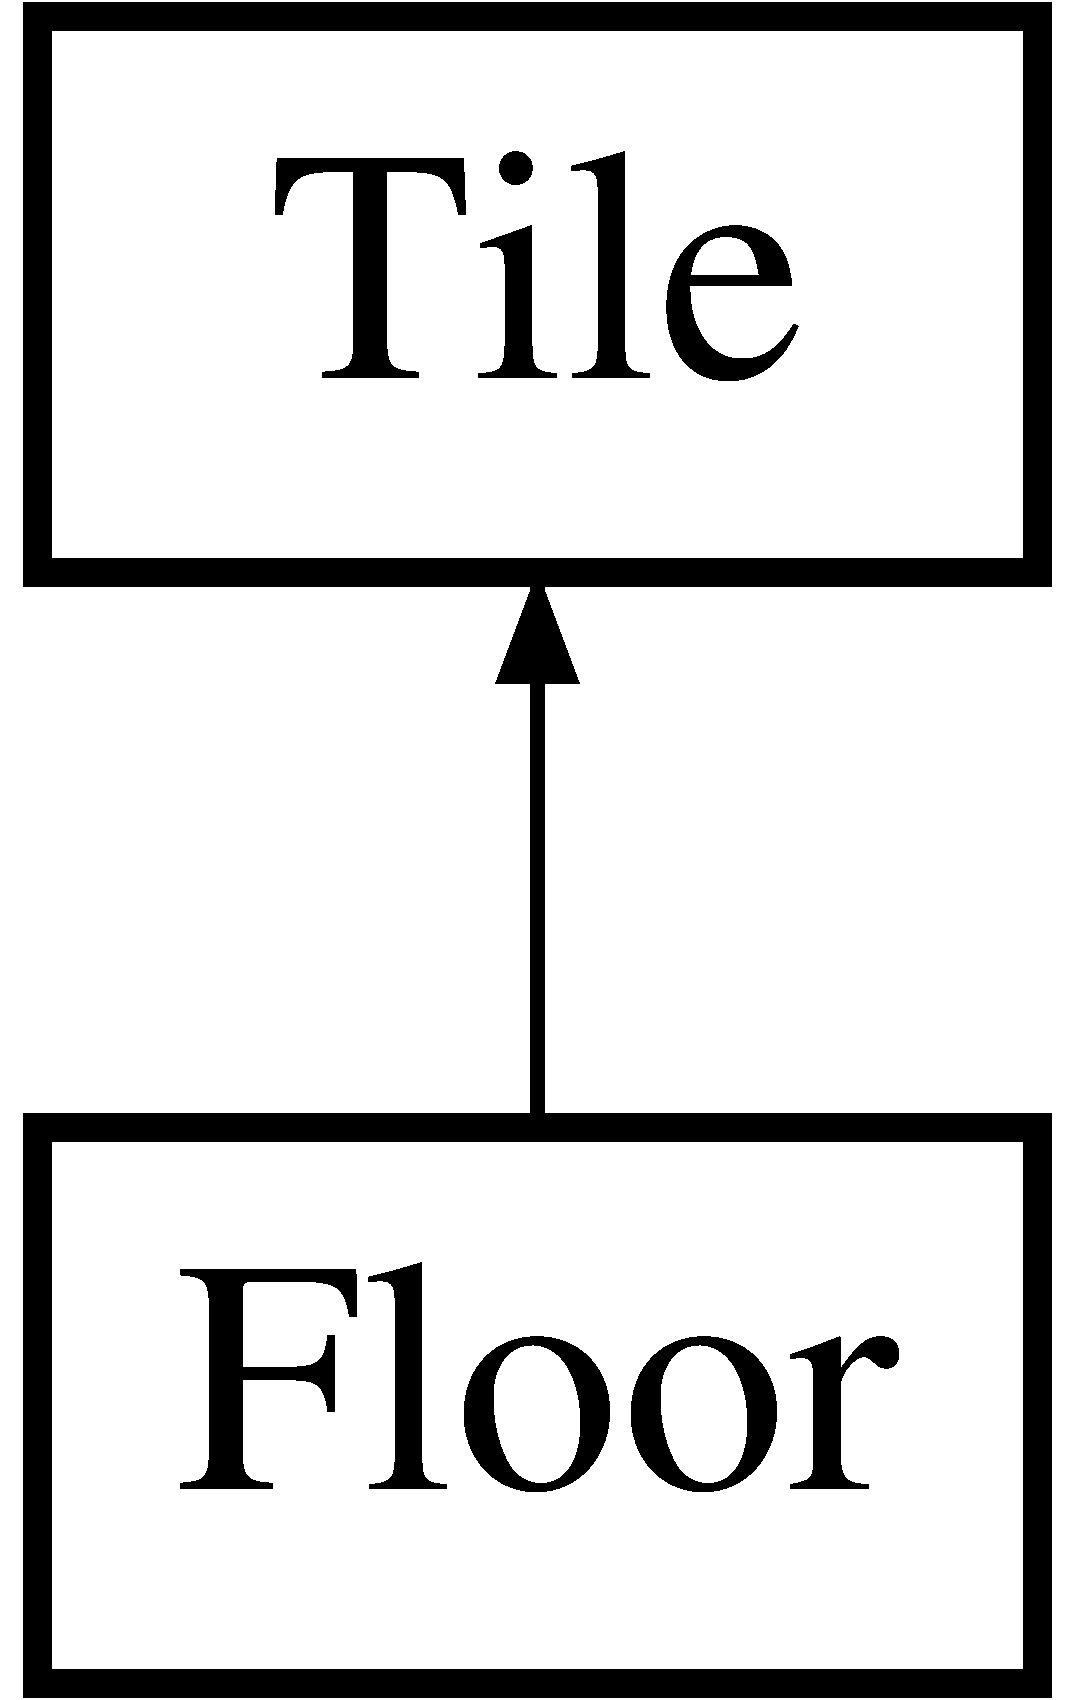
\includegraphics[height=2.000000cm]{class_floor}
\end{center}
\end{figure}
\subsection*{Public Member Functions}
\begin{DoxyCompactItemize}
\item 
\mbox{\Hypertarget{class_floor_a2a2c2380294e13ca8d9ba0b133ad4d80}\label{class_floor_a2a2c2380294e13ca8d9ba0b133ad4d80}} 
{\bfseries Floor} (sf\+::\+Vector2f pos, int type)
\item 
void \mbox{\hyperlink{class_floor_acbd296ad6187a5f1cbff67a58b525054}{load\+Image}} (int type)
\end{DoxyCompactItemize}
\subsection*{Additional Inherited Members}


\subsection{Member Function Documentation}
\mbox{\Hypertarget{class_floor_acbd296ad6187a5f1cbff67a58b525054}\label{class_floor_acbd296ad6187a5f1cbff67a58b525054}} 
\index{Floor@{Floor}!load\+Image@{load\+Image}}
\index{load\+Image@{load\+Image}!Floor@{Floor}}
\subsubsection{\texorpdfstring{load\+Image()}{loadImage()}}
{\footnotesize\ttfamily void Floor\+::load\+Image (\begin{DoxyParamCaption}\item[{int}]{type }\end{DoxyParamCaption})}

~\newline
... type determines the floor texture that is loaded

The documentation for this class was generated from the following files\+:\begin{DoxyCompactItemize}
\item 
Floor.\+h\item 
Floor.\+cpp\end{DoxyCompactItemize}

\hypertarget{class_health_power_up}{}\section{Health\+Power\+Up Class Reference}
\label{class_health_power_up}\index{Health\+Power\+Up@{Health\+Power\+Up}}
Inheritance diagram for Health\+Power\+Up\+:\begin{figure}[H]
\begin{center}
\leavevmode
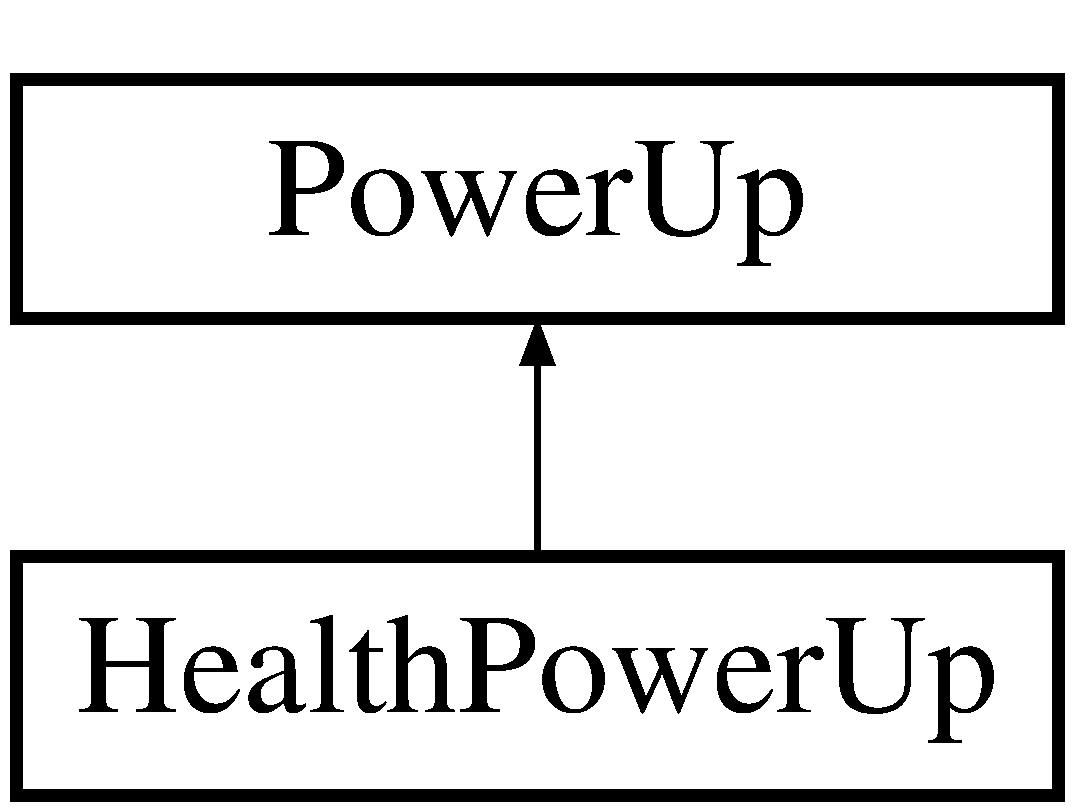
\includegraphics[height=2.000000cm]{class_health_power_up}
\end{center}
\end{figure}
\subsection*{Public Member Functions}
\begin{DoxyCompactItemize}
\item 
\mbox{\Hypertarget{class_health_power_up_a4324428f812fbf45c59b0bbaa94bdd7b}\label{class_health_power_up_a4324428f812fbf45c59b0bbaa94bdd7b}} 
{\bfseries Health\+Power\+Up} (sf\+::\+Vector2f pos)
\item 
\mbox{\Hypertarget{class_health_power_up_a71721090118d9f61b57233b85ae65eca}\label{class_health_power_up_a71721090118d9f61b57233b85ae65eca}} 
void {\bfseries check\+Collision} (\mbox{\hyperlink{class_player}{Player}} $\ast$player)
\end{DoxyCompactItemize}
\subsection*{Additional Inherited Members}


The documentation for this class was generated from the following files\+:\begin{DoxyCompactItemize}
\item 
Health\+Power\+Up.\+h\item 
Health\+Power\+Up.\+cpp\end{DoxyCompactItemize}

\hypertarget{class_nest}{}\section{Nest Class Reference}
\label{class_nest}\index{Nest@{Nest}}
\subsection*{Public Member Functions}
\begin{DoxyCompactItemize}
\item 
\mbox{\Hypertarget{class_nest_a316201617cb7b9fa85e30d350ab180d1}\label{class_nest_a316201617cb7b9fa85e30d350ab180d1}} 
{\bfseries Nest} (\mbox{\hyperlink{class_node_layout}{Node\+Layout}} \&nodes, \mbox{\hyperlink{class_player}{Player}} $\ast$player, std\+::vector$<$ \mbox{\hyperlink{class_wall}{Wall}} $\ast$$>$ \&walls)
\item 
void \mbox{\hyperlink{class_nest_a09d907a3d411da0249c7d0bb5ad7b36c}{render}} (sf\+::\+Render\+Window \&window)
\item 
void \mbox{\hyperlink{class_nest_a9af26a97505ef6ab8a0113ae6e9ddc8e}{init}} (int i)
\item 
void \mbox{\hyperlink{class_nest_a8f402fb76539074b694158a47aafe002}{update}} (float delta\+Time, \mbox{\hyperlink{class_player}{Player}} $\ast$player)
\item 
void \mbox{\hyperlink{class_nest_a01eff531c62869fdf9d41b0aea69e45f}{radar\+Render}} (sf\+::\+Render\+Window \&window)
\end{DoxyCompactItemize}


\subsection{Member Function Documentation}
\mbox{\Hypertarget{class_nest_a9af26a97505ef6ab8a0113ae6e9ddc8e}\label{class_nest_a9af26a97505ef6ab8a0113ae6e9ddc8e}} 
\index{Nest@{Nest}!init@{init}}
\index{init@{init}!Nest@{Nest}}
\subsubsection{\texorpdfstring{init()}{init()}}
{\footnotesize\ttfamily void Nest\+::init (\begin{DoxyParamCaption}\item[{int}]{i }\end{DoxyParamCaption})}

~\newline
... intialise nest obj variables\mbox{\Hypertarget{class_nest_a01eff531c62869fdf9d41b0aea69e45f}\label{class_nest_a01eff531c62869fdf9d41b0aea69e45f}} 
\index{Nest@{Nest}!radar\+Render@{radar\+Render}}
\index{radar\+Render@{radar\+Render}!Nest@{Nest}}
\subsubsection{\texorpdfstring{radar\+Render()}{radarRender()}}
{\footnotesize\ttfamily void Nest\+::radar\+Render (\begin{DoxyParamCaption}\item[{sf\+::\+Render\+Window \&}]{window }\end{DoxyParamCaption})}

... render a radar blip of the nest on minimap\mbox{\Hypertarget{class_nest_a09d907a3d411da0249c7d0bb5ad7b36c}\label{class_nest_a09d907a3d411da0249c7d0bb5ad7b36c}} 
\index{Nest@{Nest}!render@{render}}
\index{render@{render}!Nest@{Nest}}
\subsubsection{\texorpdfstring{render()}{render()}}
{\footnotesize\ttfamily void Nest\+::render (\begin{DoxyParamCaption}\item[{sf\+::\+Render\+Window \&}]{window }\end{DoxyParamCaption})}

... render the nest sprite in game world\mbox{\Hypertarget{class_nest_a8f402fb76539074b694158a47aafe002}\label{class_nest_a8f402fb76539074b694158a47aafe002}} 
\index{Nest@{Nest}!update@{update}}
\index{update@{update}!Nest@{Nest}}
\subsubsection{\texorpdfstring{update()}{update()}}
{\footnotesize\ttfamily void Nest\+::update (\begin{DoxyParamCaption}\item[{float}]{delta\+Time,  }\item[{\mbox{\hyperlink{class_player}{Player}} $\ast$}]{player }\end{DoxyParamCaption})}

... update nest and nest spawned objects

The documentation for this class was generated from the following files\+:\begin{DoxyCompactItemize}
\item 
Nest.\+h\item 
Nest.\+cpp\end{DoxyCompactItemize}

\hypertarget{class_node}{}\section{Node Class Reference}
\label{class_node}\index{Node@{Node}}
\subsection*{Public Member Functions}
\begin{DoxyCompactItemize}
\item 
\mbox{\Hypertarget{class_node_a895a106b9d0954d8c12b63ce602bc023}\label{class_node_a895a106b9d0954d8c12b63ce602bc023}} 
{\bfseries Node} (sf\+::\+Vector2f pos, int id)
\item 
\mbox{\Hypertarget{class_node_a54fc4e9571a82fa8518994f44b067f31}\label{class_node_a54fc4e9571a82fa8518994f44b067f31}} 
void {\bfseries add\+Arc} (\mbox{\hyperlink{class_node}{Node}} $\ast$n)
\item 
float \mbox{\hyperlink{class_node_a5f6014a8a8d873312eaf12303305a939}{calculate\+Arc\+Weight}} (sf\+::\+Vector2f other\+Node\+Pos)
\item 
\mbox{\Hypertarget{class_node_ae9a4a95cb9db8edaab906e655f565757}\label{class_node_ae9a4a95cb9db8edaab906e655f565757}} 
sf\+::\+Vector2f {\bfseries get\+Pos} ()
\item 
\mbox{\Hypertarget{class_node_a8dd9a1d6ac9638fd1168283ad47e5127}\label{class_node_a8dd9a1d6ac9638fd1168283ad47e5127}} 
int {\bfseries get\+ID} ()
\item 
\mbox{\Hypertarget{class_node_a68db6b1bbbf8d5e3d67b13fc1940ab7f}\label{class_node_a68db6b1bbbf8d5e3d67b13fc1940ab7f}} 
bool {\bfseries get\+Marked} ()
\item 
\mbox{\Hypertarget{class_node_acae0df9df948547644b89814f1ba1c2f}\label{class_node_acae0df9df948547644b89814f1ba1c2f}} 
void {\bfseries set\+Marked} (bool marked)
\item 
\mbox{\Hypertarget{class_node_a0a81fcd9f6bd8cf43f8ccab295411283}\label{class_node_a0a81fcd9f6bd8cf43f8ccab295411283}} 
\mbox{\hyperlink{class_node}{Node}} $\ast$ {\bfseries get\+Previous} ()
\item 
\mbox{\Hypertarget{class_node_af8c0c4e1ecf2f6a49dd899e2a57c14fb}\label{class_node_af8c0c4e1ecf2f6a49dd899e2a57c14fb}} 
void {\bfseries set\+Previous} (\mbox{\hyperlink{class_node}{Node}} $\ast$previous)
\item 
\mbox{\Hypertarget{class_node_a3e121b2968b4a04dc7a8c50fbad63045}\label{class_node_a3e121b2968b4a04dc7a8c50fbad63045}} 
float {\bfseries get\+Heuristic} ()
\item 
\mbox{\Hypertarget{class_node_a3a05e781922425fe74d2774390883d56}\label{class_node_a3a05e781922425fe74d2774390883d56}} 
void {\bfseries set\+Heuristic} (float heuristic)
\item 
\mbox{\Hypertarget{class_node_aed7dd991e4645d166a4e3770d459039a}\label{class_node_aed7dd991e4645d166a4e3770d459039a}} 
float {\bfseries get\+Cost} ()
\item 
\mbox{\Hypertarget{class_node_a9d395cc5439fc53b7d9697f44108e137}\label{class_node_a9d395cc5439fc53b7d9697f44108e137}} 
void {\bfseries set\+Cost} (float cost)
\item 
\mbox{\Hypertarget{class_node_ad341bb693aadd335d8990b48b2cbb1f7}\label{class_node_ad341bb693aadd335d8990b48b2cbb1f7}} 
std\+::list$<$ \mbox{\hyperlink{class_arc}{Arc}} $>$ \& {\bfseries get\+Arcs} ()
\end{DoxyCompactItemize}


\subsection{Member Function Documentation}
\mbox{\Hypertarget{class_node_a5f6014a8a8d873312eaf12303305a939}\label{class_node_a5f6014a8a8d873312eaf12303305a939}} 
\index{Node@{Node}!calculate\+Arc\+Weight@{calculate\+Arc\+Weight}}
\index{calculate\+Arc\+Weight@{calculate\+Arc\+Weight}!Node@{Node}}
\subsubsection{\texorpdfstring{calculate\+Arc\+Weight()}{calculateArcWeight()}}
{\footnotesize\ttfamily float Node\+::calculate\+Arc\+Weight (\begin{DoxyParamCaption}\item[{sf\+::\+Vector2f}]{other\+Node\+Pos }\end{DoxyParamCaption})}

~\newline
... weight is the distance between the nodes

The documentation for this class was generated from the following files\+:\begin{DoxyCompactItemize}
\item 
Node.\+h\item 
Node.\+cpp\end{DoxyCompactItemize}

\hypertarget{class_node_layout}{}\section{Node\+Layout Class Reference}
\label{class_node_layout}\index{Node\+Layout@{Node\+Layout}}
\subsection*{Public Member Functions}
\begin{DoxyCompactItemize}
\item 
\mbox{\Hypertarget{class_node_layout_ade973fd5d7149decaf741ab3c1f91c43}\label{class_node_layout_ade973fd5d7149decaf741ab3c1f91c43}} 
{\bfseries Node\+Layout} (std\+::vector$<$ sf\+::\+Vector2f $>$ \&node\+Data)
\item 
\mbox{\Hypertarget{class_node_layout_abab0b8ec4319ee8171c7485b4bd8b542}\label{class_node_layout_abab0b8ec4319ee8171c7485b4bd8b542}} 
int {\bfseries get\+No\+Of\+Nodes} ()
\item 
\mbox{\Hypertarget{class_node_layout_a8d764ef2d9fb8f0cefe008add406c9bc}\label{class_node_layout_a8d764ef2d9fb8f0cefe008add406c9bc}} 
\mbox{\hyperlink{class_node}{Node}} $\ast$$\ast$ {\bfseries get\+Nodes} ()
\end{DoxyCompactItemize}


The documentation for this class was generated from the following files\+:\begin{DoxyCompactItemize}
\item 
Node\+Layout.\+h\item 
Node\+Layout.\+cpp\end{DoxyCompactItemize}

\hypertarget{class_node_search_cost_comparer_a_star}{}\section{Node\+Search\+Cost\+Comparer\+A\+Star Class Reference}
\label{class_node_search_cost_comparer_a_star}\index{Node\+Search\+Cost\+Comparer\+A\+Star@{Node\+Search\+Cost\+Comparer\+A\+Star}}
\subsection*{Public Member Functions}
\begin{DoxyCompactItemize}
\item 
\mbox{\Hypertarget{class_node_search_cost_comparer_a_star_ab5af655583d46113ef1d2beae9e4dc7c}\label{class_node_search_cost_comparer_a_star_ab5af655583d46113ef1d2beae9e4dc7c}} 
bool {\bfseries operator()} (\mbox{\hyperlink{class_node}{Node}} $\ast$n1, \mbox{\hyperlink{class_node}{Node}} $\ast$n2)
\end{DoxyCompactItemize}


The documentation for this class was generated from the following file\+:\begin{DoxyCompactItemize}
\item 
Node\+Cost\+Comparer.\+h\end{DoxyCompactItemize}

\hypertarget{class_node_search_cost_comparer_u_c_s}{}\section{Node\+Search\+Cost\+Comparer\+U\+CS Class Reference}
\label{class_node_search_cost_comparer_u_c_s}\index{Node\+Search\+Cost\+Comparer\+U\+CS@{Node\+Search\+Cost\+Comparer\+U\+CS}}
\subsection*{Public Member Functions}
\begin{DoxyCompactItemize}
\item 
\mbox{\Hypertarget{class_node_search_cost_comparer_u_c_s_a8f7c857e5ba2f4b447881394214fce7f}\label{class_node_search_cost_comparer_u_c_s_a8f7c857e5ba2f4b447881394214fce7f}} 
bool {\bfseries operator()} (\mbox{\hyperlink{class_node}{Node}} $\ast$n1, \mbox{\hyperlink{class_node}{Node}} $\ast$n2)
\end{DoxyCompactItemize}


The documentation for this class was generated from the following file\+:\begin{DoxyCompactItemize}
\item 
Node\+Cost\+Comparer.\+h\end{DoxyCompactItemize}

\hypertarget{class_player}{}\section{Player Class Reference}
\label{class_player}\index{Player@{Player}}
\subsection*{Public Member Functions}
\begin{DoxyCompactItemize}
\item 
\mbox{\Hypertarget{class_player_aa6ba3005051279dc1d45ac615f197ef5}\label{class_player_aa6ba3005051279dc1d45ac615f197ef5}} 
{\bfseries Player} (std\+::vector$<$ \mbox{\hyperlink{class_wall}{Wall}} $\ast$$>$ \&walls)
\item 
\mbox{\hyperlink{class_player_a749d2c00e1fe0f5c2746f7505a58c062}{$\sim$\+Player}} ()
\item 
\mbox{\Hypertarget{class_player_a4523bf2e637fcb0e36a3f456ec397e7d}\label{class_player_a4523bf2e637fcb0e36a3f456ec397e7d}} 
void {\bfseries Init} ()
\item 
\mbox{\Hypertarget{class_player_a6a0b48c845f9c341283b5fc5a7898f9b}\label{class_player_a6a0b48c845f9c341283b5fc5a7898f9b}} 
void {\bfseries Draw} (sf\+::\+Render\+Window \&window)
\item 
\mbox{\Hypertarget{class_player_ac81962f3fcd0c78c2da40e0bfec9466f}\label{class_player_ac81962f3fcd0c78c2da40e0bfec9466f}} 
float {\bfseries get\+Fire\+Rate} ()
\item 
\mbox{\Hypertarget{class_player_a194b7082791d882887071d8d2893c5e4}\label{class_player_a194b7082791d882887071d8d2893c5e4}} 
void {\bfseries update} (float time)
\item 
\mbox{\Hypertarget{class_player_a23356f99a9de86d3d47eadb679b332dc}\label{class_player_a23356f99a9de86d3d47eadb679b332dc}} 
sf\+::\+Vector2f {\bfseries get\+Position} ()
\item 
\mbox{\Hypertarget{class_player_a34f7a992b128e39efd89821a9269b309}\label{class_player_a34f7a992b128e39efd89821a9269b309}} 
sf\+::\+Vector2f \& {\bfseries get\+Position\+Ref} ()
\item 
\mbox{\Hypertarget{class_player_aa45f751e7ba8afcd9894d57ef4813d50}\label{class_player_aa45f751e7ba8afcd9894d57ef4813d50}} 
bool {\bfseries get\+Alive} ()
\item 
\mbox{\Hypertarget{class_player_a2d1542816021d46bf0d007d57a2c7291}\label{class_player_a2d1542816021d46bf0d007d57a2c7291}} 
float {\bfseries get\+Health} ()
\item 
\mbox{\Hypertarget{class_player_a65235f2e8ad1d16ba5826cd21c16aeb5}\label{class_player_a65235f2e8ad1d16ba5826cd21c16aeb5}} 
void {\bfseries set\+Fire\+Rate} (float rate)
\item 
\mbox{\Hypertarget{class_player_ae2d4369f7701288665103149e148a669}\label{class_player_ae2d4369f7701288665103149e148a669}} 
void {\bfseries check\+Collisions} (\mbox{\hyperlink{class_wall}{Wall}} $\ast$wall, float delta\+Time)
\item 
\mbox{\Hypertarget{class_player_a876818716e936257241f6febfa6c3cc6}\label{class_player_a876818716e936257241f6febfa6c3cc6}} 
void {\bfseries set\+Position} (sf\+::\+Vector2f position)
\item 
\mbox{\Hypertarget{class_player_ae5e73c4b965ffa4d69eeedc2e31f8c5d}\label{class_player_ae5e73c4b965ffa4d69eeedc2e31f8c5d}} 
void {\bfseries set\+Alive} (bool alive)
\item 
\mbox{\Hypertarget{class_player_a2b20fb72e20c7609d903891cbf0ac3b3}\label{class_player_a2b20fb72e20c7609d903891cbf0ac3b3}} 
void {\bfseries set\+Health} (float health\+Change)
\item 
\mbox{\Hypertarget{class_player_a11dc9fd8534645977d088ca467629853}\label{class_player_a11dc9fd8534645977d088ca467629853}} 
void {\bfseries set\+Velocity} (sf\+::\+Vector2f velocity)
\item 
\mbox{\Hypertarget{class_player_ac91387d54e20b6e9286c2e2ecba5afc7}\label{class_player_ac91387d54e20b6e9286c2e2ecba5afc7}} 
void {\bfseries Draw\+Radar} (sf\+::\+Render\+Window \&window)
\item 
\mbox{\Hypertarget{class_player_a40c5ee51c931bf8c6d3f830e512d0b6a}\label{class_player_a40c5ee51c931bf8c6d3f830e512d0b6a}} 
std\+::vector$<$ \mbox{\hyperlink{class_projectile}{Projectile}} $\ast$ $>$ {\bfseries get\+Bullets} ()
\item 
\mbox{\Hypertarget{class_player_a6cfd0af7aaf2b13d65aa42f78c6085ec}\label{class_player_a6cfd0af7aaf2b13d65aa42f78c6085ec}} 
sf\+::\+Float\+Rect {\bfseries get\+Rect} ()
\item 
\mbox{\Hypertarget{class_player_a363489e11401d5a1549e315c8c8aa220}\label{class_player_a363489e11401d5a1549e315c8c8aa220}} 
sf\+::\+Vector2f {\bfseries get\+Velocity} ()
\item 
\mbox{\Hypertarget{class_player_adfa3ea6cdd232a1021cbf017010d8cde}\label{class_player_adfa3ea6cdd232a1021cbf017010d8cde}} 
bool {\bfseries get\+Shielded} ()
\item 
\mbox{\Hypertarget{class_player_a0bac13d8b70eaa143d3b95d17fbd1f91}\label{class_player_a0bac13d8b70eaa143d3b95d17fbd1f91}} 
void {\bfseries set\+Shieled} (bool shielded)
\end{DoxyCompactItemize}


\subsection{Constructor \& Destructor Documentation}
\mbox{\Hypertarget{class_player_a749d2c00e1fe0f5c2746f7505a58c062}\label{class_player_a749d2c00e1fe0f5c2746f7505a58c062}} 
\index{Player@{Player}!````~Player@{$\sim$\+Player}}
\index{````~Player@{$\sim$\+Player}!Player@{Player}}
\subsubsection{\texorpdfstring{$\sim$\+Player()}{~Player()}}
{\footnotesize\ttfamily Player\+::$\sim$\+Player (\begin{DoxyParamCaption}{ }\end{DoxyParamCaption})}

... D\+O\+X\+Y\+G\+EN T\+E\+ST B\+L\+O\+CK

The documentation for this class was generated from the following files\+:\begin{DoxyCompactItemize}
\item 
Player.\+h\item 
Player.\+cpp\end{DoxyCompactItemize}

\hypertarget{class_power_up}{}\section{Power\+Up Class Reference}
\label{class_power_up}\index{Power\+Up@{Power\+Up}}
Inheritance diagram for Power\+Up\+:\begin{figure}[H]
\begin{center}
\leavevmode
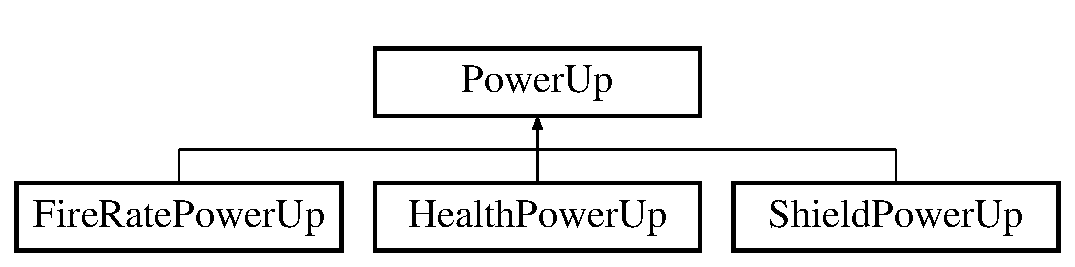
\includegraphics[height=2.000000cm]{class_power_up}
\end{center}
\end{figure}
\subsection*{Public Member Functions}
\begin{DoxyCompactItemize}
\item 
\mbox{\Hypertarget{class_power_up_aedf1753416959783efb44085b4234354}\label{class_power_up_aedf1753416959783efb44085b4234354}} 
void {\bfseries render} (sf\+::\+Render\+Window \&window)
\item 
\mbox{\Hypertarget{class_power_up_aa47b799ef32511e4bb9c7291221759c9}\label{class_power_up_aa47b799ef32511e4bb9c7291221759c9}} 
void {\bfseries check\+Collision} (\mbox{\hyperlink{class_player}{Player}} \&player)
\item 
\mbox{\Hypertarget{class_power_up_aa41037987ffd11a180652c895717cf8d}\label{class_power_up_aa41037987ffd11a180652c895717cf8d}} 
std\+::string {\bfseries get\+ID} ()
\item 
\mbox{\Hypertarget{class_power_up_a588f763447a32832f39885855d3b5f09}\label{class_power_up_a588f763447a32832f39885855d3b5f09}} 
bool {\bfseries get\+Alive} ()
\end{DoxyCompactItemize}
\subsection*{Protected Attributes}
\begin{DoxyCompactItemize}
\item 
\mbox{\Hypertarget{class_power_up_a3919e6ae0224a7da2bafdd5b54ce9f78}\label{class_power_up_a3919e6ae0224a7da2bafdd5b54ce9f78}} 
std\+::string {\bfseries id}
\item 
\mbox{\Hypertarget{class_power_up_ad8e33c49ed7402b09787fda50990f219}\label{class_power_up_ad8e33c49ed7402b09787fda50990f219}} 
sf\+::\+Vector2f {\bfseries m\+\_\+pos}
\item 
\mbox{\Hypertarget{class_power_up_ae74d9fa9fc627f00d158c42ab2a3a062}\label{class_power_up_ae74d9fa9fc627f00d158c42ab2a3a062}} 
float {\bfseries m\+\_\+width}
\item 
\mbox{\Hypertarget{class_power_up_af19e950b8cfa042872b83886a4969712}\label{class_power_up_af19e950b8cfa042872b83886a4969712}} 
float {\bfseries m\+\_\+height}
\item 
\mbox{\Hypertarget{class_power_up_aa5ada70edd6dbe5adce8ecd78b6e71a8}\label{class_power_up_aa5ada70edd6dbe5adce8ecd78b6e71a8}} 
sf\+::\+Image {\bfseries m\+\_\+image}
\item 
\mbox{\Hypertarget{class_power_up_ad1787bc5a27d9fe2c9c792b375ae236b}\label{class_power_up_ad1787bc5a27d9fe2c9c792b375ae236b}} 
sf\+::\+Texture {\bfseries m\+\_\+texture}
\item 
\mbox{\Hypertarget{class_power_up_a9fd4c1f6b35b3ff5210ad1a4384e238e}\label{class_power_up_a9fd4c1f6b35b3ff5210ad1a4384e238e}} 
sf\+::\+Sprite {\bfseries m\+\_\+sprite}
\item 
\mbox{\Hypertarget{class_power_up_a327eb8bdbc6c52111f709e8f174dbdf7}\label{class_power_up_a327eb8bdbc6c52111f709e8f174dbdf7}} 
bool {\bfseries m\+\_\+alive}
\end{DoxyCompactItemize}


The documentation for this class was generated from the following files\+:\begin{DoxyCompactItemize}
\item 
Power\+Up\+Base.\+h\item 
Power\+Up\+Base.\+cpp\end{DoxyCompactItemize}

\hypertarget{class_predator_ship}{}\section{Predator\+Ship Class Reference}
\label{class_predator_ship}\index{Predator\+Ship@{Predator\+Ship}}
\subsection*{Public Member Functions}
\begin{DoxyCompactItemize}
\item 
\mbox{\Hypertarget{class_predator_ship_a4af0d2cfa90c67811bc8cd0e3cb26e58}\label{class_predator_ship_a4af0d2cfa90c67811bc8cd0e3cb26e58}} 
{\bfseries Predator\+Ship} (sf\+::\+Vector2f pos, \mbox{\hyperlink{class_node_layout}{Node\+Layout}} \&nodes, \mbox{\hyperlink{class_player}{Player}} $\ast$player, std\+::vector$<$ \mbox{\hyperlink{class_wall}{Wall}} $\ast$$>$ \&walls)
\item 
\mbox{\Hypertarget{class_predator_ship_abd172d5ef1713de0e79e33ce7b23c13a}\label{class_predator_ship_abd172d5ef1713de0e79e33ce7b23c13a}} 
void {\bfseries render} (sf\+::\+Render\+Window \&window)
\item 
\mbox{\Hypertarget{class_predator_ship_aaecc92f60ecbaaaf2f41edbe15a458ea}\label{class_predator_ship_aaecc92f60ecbaaaf2f41edbe15a458ea}} 
void {\bfseries update} (float delta\+Time)
\item 
\mbox{\Hypertarget{class_predator_ship_a5143808a096196286fa4b3c546c183ce}\label{class_predator_ship_a5143808a096196286fa4b3c546c183ce}} 
void {\bfseries choose\+Target} (float delta\+Time)
\item 
\mbox{\Hypertarget{class_predator_ship_a941925b4c228dcbb9fae0d8f9ee8af24}\label{class_predator_ship_a941925b4c228dcbb9fae0d8f9ee8af24}} 
void {\bfseries seek} (float delta\+Time, sf\+::\+Vector2f v, float dist, bool seeking\+Player)
\item 
\mbox{\Hypertarget{class_predator_ship_aa7763a0a0b525421f672ef3e05c1b9ea}\label{class_predator_ship_aa7763a0a0b525421f672ef3e05c1b9ea}} 
void {\bfseries check\+Wall\+Collisions} (\mbox{\hyperlink{class_wall}{Wall}} $\ast$wall, float delta\+Time)
\item 
\mbox{\Hypertarget{class_predator_ship_a5b3c56caa2c17fbe78d377c0b4ad5408}\label{class_predator_ship_a5b3c56caa2c17fbe78d377c0b4ad5408}} 
void {\bfseries check\+Bullet\+Collision} (\mbox{\hyperlink{class_projectile}{Projectile}} $\ast$p)
\item 
\mbox{\Hypertarget{class_predator_ship_a68003be2e0126853481903bccb5473ed}\label{class_predator_ship_a68003be2e0126853481903bccb5473ed}} 
void {\bfseries setup\+Path} ()
\item 
\mbox{\Hypertarget{class_predator_ship_aac64b6592bb9e75c34335f0150a68d12}\label{class_predator_ship_aac64b6592bb9e75c34335f0150a68d12}} 
void {\bfseries fire\+Bullet} ()
\item 
\mbox{\Hypertarget{class_predator_ship_ad240f08c5f508a3447452d665080cf73}\label{class_predator_ship_ad240f08c5f508a3447452d665080cf73}} 
void {\bfseries normalise} (sf\+::\+Vector2f \&v)
\item 
\mbox{\Hypertarget{class_predator_ship_acaef1f914f1cd32445977927fd4f2d85}\label{class_predator_ship_acaef1f914f1cd32445977927fd4f2d85}} 
float {\bfseries calculate\+Magnitude} (sf\+::\+Vector2f v)
\item 
\mbox{\Hypertarget{class_predator_ship_a8000ba5e3ef3024de39cc7763048af72}\label{class_predator_ship_a8000ba5e3ef3024de39cc7763048af72}} 
float {\bfseries calculate\+Magnitude} (sf\+::\+Vector2f v1, sf\+::\+Vector2f v2)
\item 
\mbox{\Hypertarget{class_predator_ship_a91fdb3bab56c53417c0fa33237768f64}\label{class_predator_ship_a91fdb3bab56c53417c0fa33237768f64}} 
sf\+::\+Float\+Rect {\bfseries get\+Rect} ()
\item 
\mbox{\Hypertarget{class_predator_ship_a4f32416e9d9175ec61bab70008ad709f}\label{class_predator_ship_a4f32416e9d9175ec61bab70008ad709f}} 
void {\bfseries render\+Radar} (sf\+::\+Render\+Window \&window)
\item 
\mbox{\Hypertarget{class_predator_ship_a7a85b35820234fa6cefa69b6108498e7}\label{class_predator_ship_a7a85b35820234fa6cefa69b6108498e7}} 
void {\bfseries check\+Player\+Bullet\+Coll} ()
\item 
\mbox{\Hypertarget{class_predator_ship_aae0461ff2cd58e4b6249d3375b297281}\label{class_predator_ship_aae0461ff2cd58e4b6249d3375b297281}} 
bool {\bfseries get\+Alive} ()
\end{DoxyCompactItemize}


The documentation for this class was generated from the following files\+:\begin{DoxyCompactItemize}
\item 
Predator\+Ship.\+h\item 
Predator\+Ship.\+cpp\end{DoxyCompactItemize}

\hypertarget{class_projectile}{}\section{Projectile Class Reference}
\label{class_projectile}\index{Projectile@{Projectile}}
\subsection*{Public Member Functions}
\begin{DoxyCompactItemize}
\item 
\mbox{\Hypertarget{class_projectile_aa89daaa748dc847bd0ed4c5b131e18c1}\label{class_projectile_aa89daaa748dc847bd0ed4c5b131e18c1}} 
{\bfseries Projectile} (sf\+::\+Vector2f pos, float rot, float mag, sf\+::\+Vector2f velocity)
\item 
\mbox{\Hypertarget{class_projectile_a9b1fe47f547a234439f87adc8759df8d}\label{class_projectile_a9b1fe47f547a234439f87adc8759df8d}} 
void {\bfseries initialise} (sf\+::\+Vector2f pos, float rot, sf\+::\+Vector2f velocity)
\item 
\mbox{\Hypertarget{class_projectile_a5bc646de87829b911d6817a6478c353e}\label{class_projectile_a5bc646de87829b911d6817a6478c353e}} 
void {\bfseries update} (float delta\+Time)
\item 
\mbox{\Hypertarget{class_projectile_a88ed5be04ec9eddeb83deb201607368c}\label{class_projectile_a88ed5be04ec9eddeb83deb201607368c}} 
sf\+::\+Vector2f {\bfseries get\+Position} ()
\item 
\mbox{\Hypertarget{class_projectile_acdcf53a4c078135f7d7cd86871c9bb91}\label{class_projectile_acdcf53a4c078135f7d7cd86871c9bb91}} 
bool {\bfseries get\+Alive} ()
\item 
\mbox{\Hypertarget{class_projectile_a983d5d433a3dc8c6124e7efe2a57c635}\label{class_projectile_a983d5d433a3dc8c6124e7efe2a57c635}} 
float {\bfseries get\+Health} ()
\item 
\mbox{\Hypertarget{class_projectile_a92bcfb9a5b0fdcdaf73bf38502f22304}\label{class_projectile_a92bcfb9a5b0fdcdaf73bf38502f22304}} 
sf\+::\+Vector2f {\bfseries get\+Velocity} ()
\item 
\mbox{\Hypertarget{class_projectile_aebced9bbe25d8b9a3b214a12201a04d9}\label{class_projectile_aebced9bbe25d8b9a3b214a12201a04d9}} 
float {\bfseries get\+Orient} (float orientation, sf\+::\+Vector2f velocity, sf\+::\+Vector2f target)
\item 
\mbox{\Hypertarget{class_projectile_afb7d5c794f26e495ccbc5b597bb01246}\label{class_projectile_afb7d5c794f26e495ccbc5b597bb01246}} 
float {\bfseries get\+Width} ()
\item 
\mbox{\Hypertarget{class_projectile_a70d55ea52a1d6cdaf74c894d412597d1}\label{class_projectile_a70d55ea52a1d6cdaf74c894d412597d1}} 
float {\bfseries get\+Height} ()
\item 
\mbox{\Hypertarget{class_projectile_ae07f879ff7091e007f89e1e875f08962}\label{class_projectile_ae07f879ff7091e007f89e1e875f08962}} 
void {\bfseries set\+Position} (sf\+::\+Vector2f position)
\item 
\mbox{\Hypertarget{class_projectile_a7125bb834b93eb0dbe6484c015949e80}\label{class_projectile_a7125bb834b93eb0dbe6484c015949e80}} 
void {\bfseries set\+Alive} (bool alive)
\item 
\mbox{\Hypertarget{class_projectile_a98891d8de7607df133f975ec8e249ccf}\label{class_projectile_a98891d8de7607df133f975ec8e249ccf}} 
void {\bfseries set\+Velocity} (sf\+::\+Vector2f velocity)
\item 
\mbox{\Hypertarget{class_projectile_a0c13be2f57f656bae015fa3ecfffa572}\label{class_projectile_a0c13be2f57f656bae015fa3ecfffa572}} 
void {\bfseries Draw} (sf\+::\+Render\+Window \&window)
\end{DoxyCompactItemize}
\subsection*{Public Attributes}
\begin{DoxyCompactItemize}
\item 
\mbox{\Hypertarget{class_projectile_ada05bf23fbcb757cd7121dec3d0a72bd}\label{class_projectile_ada05bf23fbcb757cd7121dec3d0a72bd}} 
sf\+::\+Time {\bfseries lifetime}
\item 
\mbox{\Hypertarget{class_projectile_a2a4fb9a99683ea017ca05a8a0d8a670c}\label{class_projectile_a2a4fb9a99683ea017ca05a8a0d8a670c}} 
sf\+::\+Clock {\bfseries life\+Clock}
\end{DoxyCompactItemize}


The documentation for this class was generated from the following files\+:\begin{DoxyCompactItemize}
\item 
Projectile.\+h\item 
Projectile.\+cpp\end{DoxyCompactItemize}

\hypertarget{class_seeker_missile}{}\section{Seeker\+Missile Class Reference}
\label{class_seeker_missile}\index{Seeker\+Missile@{Seeker\+Missile}}
\subsection*{Public Member Functions}
\begin{DoxyCompactItemize}
\item 
\mbox{\Hypertarget{class_seeker_missile_a09c20c51520a2ee6c3282d7284ec1528}\label{class_seeker_missile_a09c20c51520a2ee6c3282d7284ec1528}} 
void {\bfseries initialise} (int i, sf\+::\+Vector2f pos)
\item 
\mbox{\Hypertarget{class_seeker_missile_af3baaea8b9680a9acb037a1596d9403b}\label{class_seeker_missile_af3baaea8b9680a9acb037a1596d9403b}} 
void {\bfseries update} (float i, \mbox{\hyperlink{class_player}{Player}} $\ast$player, float delta\+Time)
\item 
\mbox{\Hypertarget{class_seeker_missile_aec565a6d030044f0b96b6b9e599aff80}\label{class_seeker_missile_aec565a6d030044f0b96b6b9e599aff80}} 
sf\+::\+Vector2f {\bfseries get\+Position} ()
\item 
\mbox{\Hypertarget{class_seeker_missile_ae60ac129a3cc0810b98e8284b3d622af}\label{class_seeker_missile_ae60ac129a3cc0810b98e8284b3d622af}} 
bool {\bfseries get\+Alive} ()
\item 
\mbox{\Hypertarget{class_seeker_missile_a34ee6daa06745c921bc27e13e0ac8150}\label{class_seeker_missile_a34ee6daa06745c921bc27e13e0ac8150}} 
float {\bfseries get\+Health} ()
\item 
\mbox{\Hypertarget{class_seeker_missile_a21ff15f78ec3ceb191735b13b2f86aeb}\label{class_seeker_missile_a21ff15f78ec3ceb191735b13b2f86aeb}} 
sf\+::\+Vector2f {\bfseries get\+Velocity} ()
\item 
\mbox{\Hypertarget{class_seeker_missile_aaead4b6d7f967a6a7de3b53a4b5b425a}\label{class_seeker_missile_aaead4b6d7f967a6a7de3b53a4b5b425a}} 
void {\bfseries Flee} (sf\+::\+Vector2f target)
\item 
\mbox{\Hypertarget{class_seeker_missile_a1fe0f447573c340c2a11c0313ebf9ea2}\label{class_seeker_missile_a1fe0f447573c340c2a11c0313ebf9ea2}} 
void {\bfseries Seek} (sf\+::\+Vector2f target, \mbox{\hyperlink{class_player}{Player}} $\ast$player)
\item 
\mbox{\Hypertarget{class_seeker_missile_a0cf52290284abf389c795efc9a1db3d1}\label{class_seeker_missile_a0cf52290284abf389c795efc9a1db3d1}} 
void {\bfseries Wander} (sf\+::\+Vector2f target)
\item 
\mbox{\Hypertarget{class_seeker_missile_afd7d8339af95452635f7ed84373c66b0}\label{class_seeker_missile_afd7d8339af95452635f7ed84373c66b0}} 
float {\bfseries Arrive} (sf\+::\+Vector2f target, \mbox{\hyperlink{class_player}{Player}} $\ast$player)
\item 
\mbox{\Hypertarget{class_seeker_missile_aa730a51000b8b61385d5725febda4962}\label{class_seeker_missile_aa730a51000b8b61385d5725febda4962}} 
void {\bfseries rotate\+Over\+Time} (sf\+::\+Vector2f vec, sf\+::\+Time timespan, sf\+::\+Time elapsed\+Time\+Since\+Start)
\item 
\mbox{\Hypertarget{class_seeker_missile_a9ab2ce9cc84d0cd47a6be437025dd0d3}\label{class_seeker_missile_a9ab2ce9cc84d0cd47a6be437025dd0d3}} 
void {\bfseries set\+Position} (sf\+::\+Vector2f position)
\item 
\mbox{\Hypertarget{class_seeker_missile_ac0d126a95002d312305b51f3625a728b}\label{class_seeker_missile_ac0d126a95002d312305b51f3625a728b}} 
void {\bfseries set\+Alive} (bool alive)
\item 
\mbox{\Hypertarget{class_seeker_missile_abdafa685dda98c78488c54629d427d58}\label{class_seeker_missile_abdafa685dda98c78488c54629d427d58}} 
void {\bfseries set\+Health} (float health\+Change)
\item 
\mbox{\Hypertarget{class_seeker_missile_a9621e4dca70af019f083681c6ee1d6c2}\label{class_seeker_missile_a9621e4dca70af019f083681c6ee1d6c2}} 
void {\bfseries set\+Velocity} (sf\+::\+Vector2f velocity)
\item 
\mbox{\Hypertarget{class_seeker_missile_acb47a64a571ad9660ebe47ebd1595d20}\label{class_seeker_missile_acb47a64a571ad9660ebe47ebd1595d20}} 
float {\bfseries get\+Orient} (float orientation, sf\+::\+Vector2f velocity, sf\+::\+Vector2f target)
\item 
\mbox{\Hypertarget{class_seeker_missile_a8744918a81a590920c2555ac68dac04c}\label{class_seeker_missile_a8744918a81a590920c2555ac68dac04c}} 
void {\bfseries Draw} (sf\+::\+Render\+Window \&window)
\end{DoxyCompactItemize}
\subsection*{Public Attributes}
\begin{DoxyCompactItemize}
\item 
\mbox{\Hypertarget{class_seeker_missile_a22f333589b0567df4a2442f892a4e530}\label{class_seeker_missile_a22f333589b0567df4a2442f892a4e530}} 
sf\+::\+Time {\bfseries lifetime}
\item 
\mbox{\Hypertarget{class_seeker_missile_a1c589b64ef67acfb3881c80067edcd4a}\label{class_seeker_missile_a1c589b64ef67acfb3881c80067edcd4a}} 
sf\+::\+Clock {\bfseries life\+Clock}
\end{DoxyCompactItemize}


The documentation for this class was generated from the following files\+:\begin{DoxyCompactItemize}
\item 
Seeker\+Missile.\+h\item 
Seeker\+Missile.\+cpp\end{DoxyCompactItemize}

\hypertarget{class_shield_power_up}{}\section{Shield\+Power\+Up Class Reference}
\label{class_shield_power_up}\index{Shield\+Power\+Up@{Shield\+Power\+Up}}
Inheritance diagram for Shield\+Power\+Up\+:\begin{figure}[H]
\begin{center}
\leavevmode
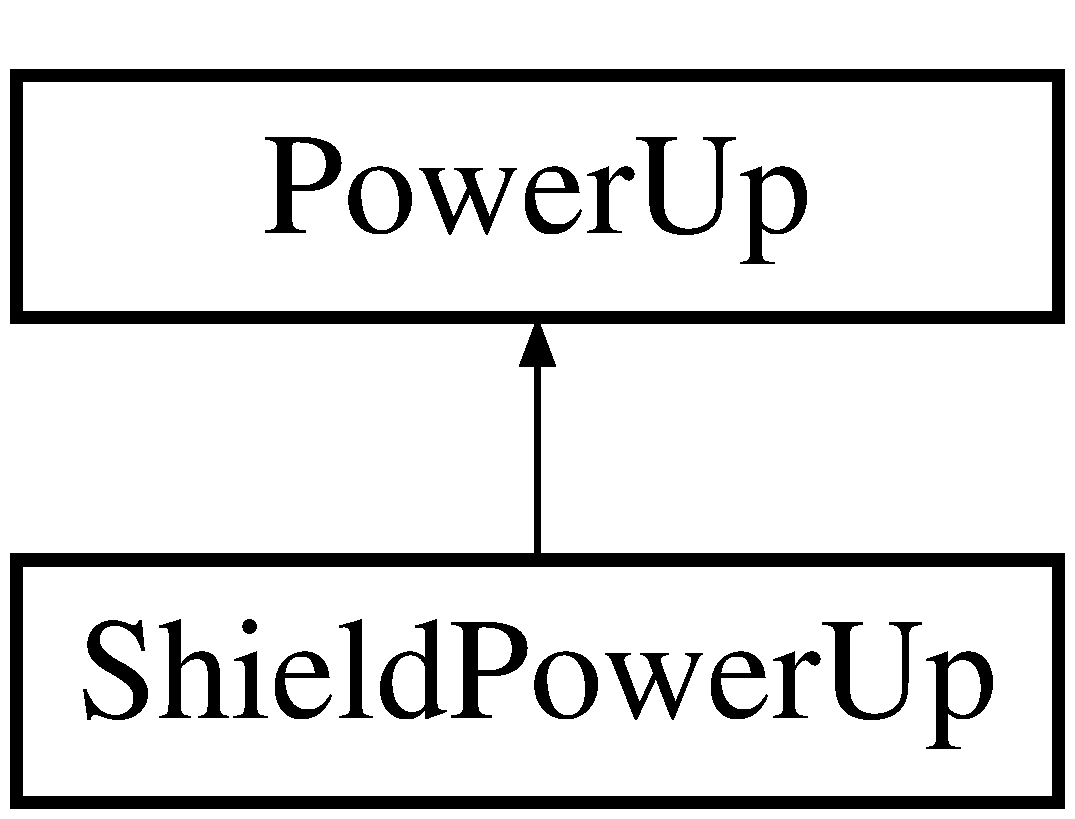
\includegraphics[height=2.000000cm]{class_shield_power_up}
\end{center}
\end{figure}
\subsection*{Public Member Functions}
\begin{DoxyCompactItemize}
\item 
\mbox{\Hypertarget{class_shield_power_up_ac41f988ed81ed73f22cf83fbf1481964}\label{class_shield_power_up_ac41f988ed81ed73f22cf83fbf1481964}} 
{\bfseries Shield\+Power\+Up} (sf\+::\+Vector2f pos)
\item 
\mbox{\Hypertarget{class_shield_power_up_a4055c8c6d5412da1c338baca3658a301}\label{class_shield_power_up_a4055c8c6d5412da1c338baca3658a301}} 
void {\bfseries check\+Collision} (\mbox{\hyperlink{class_player}{Player}} $\ast$player)
\end{DoxyCompactItemize}
\subsection*{Additional Inherited Members}


The documentation for this class was generated from the following files\+:\begin{DoxyCompactItemize}
\item 
Shield\+Power\+Up.\+h\item 
Shield\+Power\+Up.\+cpp\end{DoxyCompactItemize}

\hypertarget{class_space_station}{}\section{Space\+Station Class Reference}
\label{class_space_station}\index{Space\+Station@{Space\+Station}}
\subsection*{Public Member Functions}
\begin{DoxyCompactItemize}
\item 
\mbox{\hyperlink{class_space_station_ab8582f38baf13f990b87cf42d7c2293c}{Space\+Station}} ()
\item 
void \mbox{\hyperlink{class_space_station_a824f72a1cc84e640f8db8be290227cbe}{render}} (sf\+::\+Render\+Window \&window)
\item 
\mbox{\Hypertarget{class_space_station_a448dc37ced5e9954461899ddebc8a69e}\label{class_space_station_a448dc37ced5e9954461899ddebc8a69e}} 
\mbox{\hyperlink{class_node_layout}{Node\+Layout}} \& {\bfseries get\+Node\+Layout} ()
\item 
\mbox{\Hypertarget{class_space_station_a3d7dd73588dac0f1c9ae662526c7e29f}\label{class_space_station_a3d7dd73588dac0f1c9ae662526c7e29f}} 
std\+::vector$<$ \mbox{\hyperlink{class_wall}{Wall}} $\ast$ $>$ \& {\bfseries get\+Walls} ()
\item 
\mbox{\Hypertarget{class_space_station_a8a15fe86e9b1639d320951e5914e8120}\label{class_space_station_a8a15fe86e9b1639d320951e5914e8120}} 
std\+::vector$<$ \mbox{\hyperlink{class_floor}{Floor}} $\ast$ $>$ {\bfseries get\+Floors} ()
\item 
\mbox{\Hypertarget{class_space_station_a32f408563c74832a7e5b86f2f2edd0d4}\label{class_space_station_a32f408563c74832a7e5b86f2f2edd0d4}} 
std\+::vector$<$ \mbox{\hyperlink{class_power_up}{Power\+Up}} $\ast$ $>$ \& {\bfseries get\+Power\+Ups} ()
\end{DoxyCompactItemize}


\subsection{Constructor \& Destructor Documentation}
\mbox{\Hypertarget{class_space_station_ab8582f38baf13f990b87cf42d7c2293c}\label{class_space_station_ab8582f38baf13f990b87cf42d7c2293c}} 
\index{Space\+Station@{Space\+Station}!Space\+Station@{Space\+Station}}
\index{Space\+Station@{Space\+Station}!Space\+Station@{Space\+Station}}
\subsubsection{\texorpdfstring{Space\+Station()}{SpaceStation()}}
{\footnotesize\ttfamily Space\+Station\+::\+Space\+Station (\begin{DoxyParamCaption}{ }\end{DoxyParamCaption})}

~\newline
... // constructor to set up map tiles

\subsection{Member Function Documentation}
\mbox{\Hypertarget{class_space_station_a824f72a1cc84e640f8db8be290227cbe}\label{class_space_station_a824f72a1cc84e640f8db8be290227cbe}} 
\index{Space\+Station@{Space\+Station}!render@{render}}
\index{render@{render}!Space\+Station@{Space\+Station}}
\subsubsection{\texorpdfstring{render()}{render()}}
{\footnotesize\ttfamily void Space\+Station\+::render (\begin{DoxyParamCaption}\item[{sf\+::\+Render\+Window \&}]{window }\end{DoxyParamCaption})}

~\newline
... // render tiles in game world

The documentation for this class was generated from the following files\+:\begin{DoxyCompactItemize}
\item 
Space\+Station.\+h\item 
Space\+Station.\+cpp\end{DoxyCompactItemize}

\hypertarget{class_sweeper_boid}{}\section{Sweeper\+Boid Class Reference}
\label{class_sweeper_boid}\index{Sweeper\+Boid@{Sweeper\+Boid}}
\subsection*{Public Member Functions}
\begin{DoxyCompactItemize}
\item 
\mbox{\hyperlink{class_sweeper_boid_a1beb859233e11e9656ce5b501ee739d0}{Sweeper\+Boid}} (\mbox{\hyperlink{class_node_layout}{Node\+Layout}} \&nodes, \mbox{\hyperlink{class_player}{Player}} $\ast$player, std\+::vector$<$ \mbox{\hyperlink{class_wall}{Wall}} $\ast$$>$ \&walls, std\+::vector$<$ \mbox{\hyperlink{class_worker}{Worker}} $\ast$$>$ \&workers, int path\+No)
\item 
\mbox{\Hypertarget{class_sweeper_boid_a060fdd3341601b642bec5f298525acc3}\label{class_sweeper_boid_a060fdd3341601b642bec5f298525acc3}} 
void {\bfseries render} (sf\+::\+Render\+Window \&window)
\item 
\mbox{\Hypertarget{class_sweeper_boid_ace06cb07304ac46df07e70ff77cec967}\label{class_sweeper_boid_ace06cb07304ac46df07e70ff77cec967}} 
void {\bfseries update} (float delta\+Time)
\item 
\mbox{\Hypertarget{class_sweeper_boid_aa7fc2ba9acff8abd55af1872d734181d}\label{class_sweeper_boid_aa7fc2ba9acff8abd55af1872d734181d}} 
void {\bfseries choose\+Target} ()
\item 
\mbox{\Hypertarget{class_sweeper_boid_ab88569c90abe8ffea6d199d1c4d25fdf}\label{class_sweeper_boid_ab88569c90abe8ffea6d199d1c4d25fdf}} 
void {\bfseries seek} (float delta\+Time, sf\+::\+Vector2f v, float dist, bool seeking\+Worker)
\item 
\mbox{\Hypertarget{class_sweeper_boid_a718a85eabf5b4e7e8361ae0e4fd70fec}\label{class_sweeper_boid_a718a85eabf5b4e7e8361ae0e4fd70fec}} 
void {\bfseries check\+Wall\+Collisions} (\mbox{\hyperlink{class_wall}{Wall}} $\ast$wall, float delta\+Time)
\item 
\mbox{\Hypertarget{class_sweeper_boid_a9e38c7720c06e898a8e1217184ea32fa}\label{class_sweeper_boid_a9e38c7720c06e898a8e1217184ea32fa}} 
void {\bfseries choose\+Behaviour} ()
\item 
void \mbox{\hyperlink{class_sweeper_boid_acf5db66e58a6c7c9322953e2abd4214c}{check\+Bullet\+Collision}} (\mbox{\hyperlink{class_projectile}{Projectile}} $\ast$p)
\item 
\mbox{\Hypertarget{class_sweeper_boid_ae2e5c623aa6d8675eddf5ba2470539cb}\label{class_sweeper_boid_ae2e5c623aa6d8675eddf5ba2470539cb}} 
void {\bfseries setup\+Patrol} (int path\+No)
\item 
\mbox{\Hypertarget{class_sweeper_boid_ad0bba56551cd9fa781c8d04fc6c1c361}\label{class_sweeper_boid_ad0bba56551cd9fa781c8d04fc6c1c361}} 
void {\bfseries patrol} (float delta\+Time)
\item 
\mbox{\Hypertarget{class_sweeper_boid_a7342a56a2441de343c42eee27728857b}\label{class_sweeper_boid_a7342a56a2441de343c42eee27728857b}} 
void {\bfseries setup\+Seek\+Path} ()
\item 
\mbox{\Hypertarget{class_sweeper_boid_abe27341c9ac74d29d6c35960f8e5d873}\label{class_sweeper_boid_abe27341c9ac74d29d6c35960f8e5d873}} 
void {\bfseries abduct} (float delta\+Time)
\item 
\mbox{\Hypertarget{class_sweeper_boid_abc52f564c73c8083921653477e327700}\label{class_sweeper_boid_abc52f564c73c8083921653477e327700}} 
void {\bfseries setup\+Return\+Path} ()
\item 
\mbox{\Hypertarget{class_sweeper_boid_a6ecd02773c903b57b25aec9fd415b184}\label{class_sweeper_boid_a6ecd02773c903b57b25aec9fd415b184}} 
void {\bfseries return\+To\+Patrol} (float delta\+Time)
\item 
\mbox{\Hypertarget{class_sweeper_boid_a39023985f11037212b4c40f55cecf306}\label{class_sweeper_boid_a39023985f11037212b4c40f55cecf306}} 
void {\bfseries setup\+Flee\+Path} (float min\+Dist)
\item 
\mbox{\Hypertarget{class_sweeper_boid_a475e95d6f874ebce01b6904bd85193ea}\label{class_sweeper_boid_a475e95d6f874ebce01b6904bd85193ea}} 
void {\bfseries flee} (float delta\+Time, sf\+::\+Vector2f v)
\item 
\mbox{\Hypertarget{class_sweeper_boid_a065ded798eb1b37ab4cc9944824795c9}\label{class_sweeper_boid_a065ded798eb1b37ab4cc9944824795c9}} 
void {\bfseries normalise} (sf\+::\+Vector2f \&v)
\item 
\mbox{\Hypertarget{class_sweeper_boid_a91e883fffbab6b77c509cd4a482a8137}\label{class_sweeper_boid_a91e883fffbab6b77c509cd4a482a8137}} 
float {\bfseries calculate\+Magnitude} (sf\+::\+Vector2f v)
\item 
\mbox{\Hypertarget{class_sweeper_boid_a148901a7afea04b6bab331053e15655a}\label{class_sweeper_boid_a148901a7afea04b6bab331053e15655a}} 
float {\bfseries calculate\+Magnitude} (sf\+::\+Vector2f v1, sf\+::\+Vector2f v2)
\item 
\mbox{\Hypertarget{class_sweeper_boid_af33a3a064c32fe372475b9e3722f9630}\label{class_sweeper_boid_af33a3a064c32fe372475b9e3722f9630}} 
bool {\bfseries get\+Alive} ()
\item 
\mbox{\Hypertarget{class_sweeper_boid_a1b7a0488528da4843f0821b555b14d0f}\label{class_sweeper_boid_a1b7a0488528da4843f0821b555b14d0f}} 
std\+::vector$<$ int $>$ {\bfseries get\+Indexes\+Of\+Abducted} ()
\end{DoxyCompactItemize}


\subsection{Constructor \& Destructor Documentation}
\mbox{\Hypertarget{class_sweeper_boid_a1beb859233e11e9656ce5b501ee739d0}\label{class_sweeper_boid_a1beb859233e11e9656ce5b501ee739d0}} 
\index{Sweeper\+Boid@{Sweeper\+Boid}!Sweeper\+Boid@{Sweeper\+Boid}}
\index{Sweeper\+Boid@{Sweeper\+Boid}!Sweeper\+Boid@{Sweeper\+Boid}}
\subsubsection{\texorpdfstring{Sweeper\+Boid()}{SweeperBoid()}}
{\footnotesize\ttfamily Sweeper\+Boid\+::\+Sweeper\+Boid (\begin{DoxyParamCaption}\item[{\mbox{\hyperlink{class_node_layout}{Node\+Layout}} \&}]{nodes,  }\item[{\mbox{\hyperlink{class_player}{Player}} $\ast$}]{player,  }\item[{std\+::vector$<$ \mbox{\hyperlink{class_wall}{Wall}} $\ast$$>$ \&}]{walls,  }\item[{std\+::vector$<$ \mbox{\hyperlink{class_worker}{Worker}} $\ast$$>$ \&}]{workers,  }\item[{int}]{path\+No }\end{DoxyParamCaption})}

... // initialises sweeper boid

\subsection{Member Function Documentation}
\mbox{\Hypertarget{class_sweeper_boid_acf5db66e58a6c7c9322953e2abd4214c}\label{class_sweeper_boid_acf5db66e58a6c7c9322953e2abd4214c}} 
\index{Sweeper\+Boid@{Sweeper\+Boid}!check\+Bullet\+Collision@{check\+Bullet\+Collision}}
\index{check\+Bullet\+Collision@{check\+Bullet\+Collision}!Sweeper\+Boid@{Sweeper\+Boid}}
\subsubsection{\texorpdfstring{check\+Bullet\+Collision()}{checkBulletCollision()}}
{\footnotesize\ttfamily void Sweeper\+Boid\+::check\+Bullet\+Collision (\begin{DoxyParamCaption}\item[{\mbox{\hyperlink{class_projectile}{Projectile}} $\ast$}]{p }\end{DoxyParamCaption})}

... // checks collision between sweeper and player bullets

The documentation for this class was generated from the following files\+:\begin{DoxyCompactItemize}
\item 
Sweeper\+Boid.\+h\item 
Sweeper\+Boid.\+cpp\end{DoxyCompactItemize}

\hypertarget{class_tile}{}\section{Tile Class Reference}
\label{class_tile}\index{Tile@{Tile}}
Inheritance diagram for Tile\+:\begin{figure}[H]
\begin{center}
\leavevmode
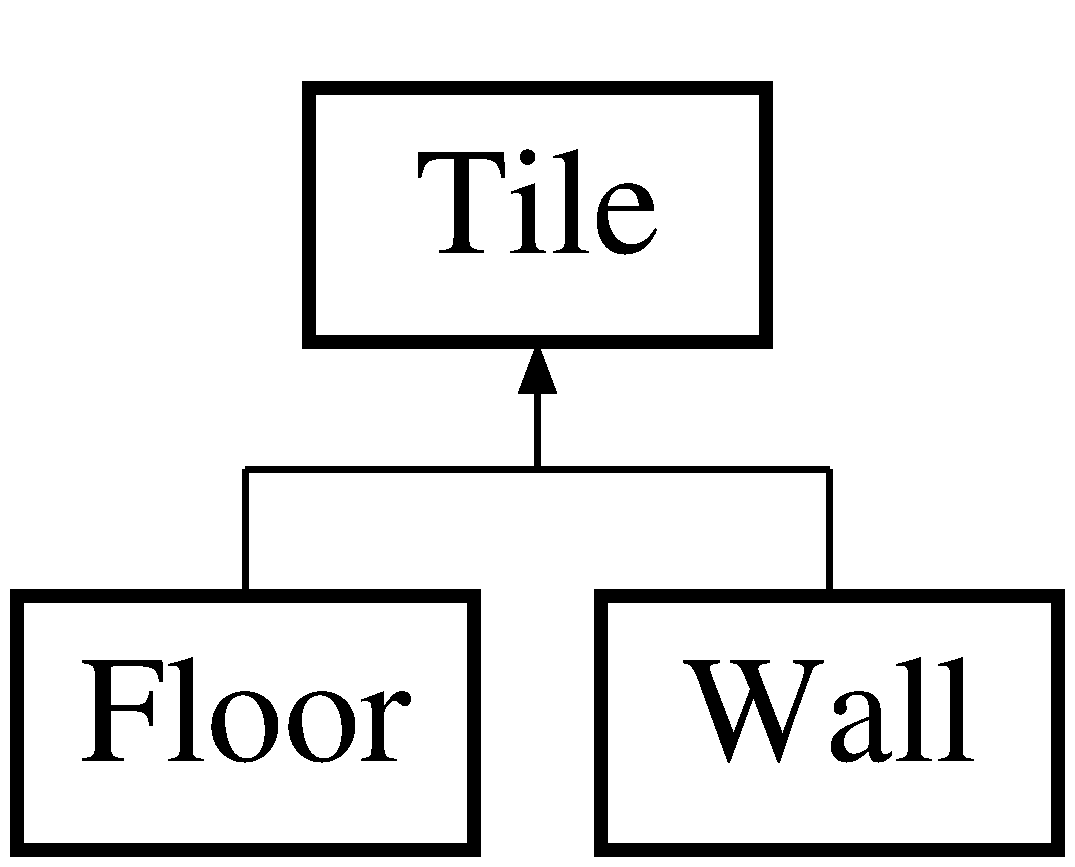
\includegraphics[height=2.000000cm]{class_tile}
\end{center}
\end{figure}
\subsection*{Public Member Functions}
\begin{DoxyCompactItemize}
\item 
\mbox{\Hypertarget{class_tile_aa725e7733d68aa1bff21e5478e7a4657}\label{class_tile_aa725e7733d68aa1bff21e5478e7a4657}} 
{\bfseries Tile} (sf\+::\+Vector2f pos)
\item 
\mbox{\Hypertarget{class_tile_a75f7d0d215ea908c553b24fa0d3621d4}\label{class_tile_a75f7d0d215ea908c553b24fa0d3621d4}} 
void {\bfseries load\+Image} ()
\item 
\mbox{\Hypertarget{class_tile_a57444de210a362d359197d5a6b5e16e9}\label{class_tile_a57444de210a362d359197d5a6b5e16e9}} 
void {\bfseries render} (sf\+::\+Render\+Window \&window)
\item 
\mbox{\Hypertarget{class_tile_ae2e177d16e7d6268c0858d660b5784f4}\label{class_tile_ae2e177d16e7d6268c0858d660b5784f4}} 
sf\+::\+Vector2f {\bfseries get\+Pos} ()
\item 
\mbox{\Hypertarget{class_tile_a8d2243b5b2ae8ca6305aae05f709c09b}\label{class_tile_a8d2243b5b2ae8ca6305aae05f709c09b}} 
sf\+::\+Vector2f {\bfseries get\+Center} ()
\item 
\mbox{\Hypertarget{class_tile_a0900b10be1e58a6edefefdeb8ac495dc}\label{class_tile_a0900b10be1e58a6edefefdeb8ac495dc}} 
float {\bfseries get\+Right} ()
\item 
\mbox{\Hypertarget{class_tile_aa5dd2afb7ecead62f1553ef90eb45c8b}\label{class_tile_aa5dd2afb7ecead62f1553ef90eb45c8b}} 
float {\bfseries get\+Width} ()
\item 
\mbox{\Hypertarget{class_tile_abe606f06c3d9bbb78eeb6c24f029695e}\label{class_tile_abe606f06c3d9bbb78eeb6c24f029695e}} 
float {\bfseries get\+Bottom} ()
\item 
\mbox{\Hypertarget{class_tile_a5411a2b368fe4eb206cb13d97642c764}\label{class_tile_a5411a2b368fe4eb206cb13d97642c764}} 
float {\bfseries get\+Height} ()
\item 
\mbox{\Hypertarget{class_tile_a16069b420eef8311589ade1eca42ed64}\label{class_tile_a16069b420eef8311589ade1eca42ed64}} 
sf\+::\+Float\+Rect {\bfseries get\+Rect} ()
\item 
\mbox{\Hypertarget{class_tile_af3dec632de42f9e9784af0dce462837c}\label{class_tile_af3dec632de42f9e9784af0dce462837c}} 
sf\+::\+Sprite {\bfseries get\+Sprite} ()
\end{DoxyCompactItemize}
\subsection*{Protected Attributes}
\begin{DoxyCompactItemize}
\item 
\mbox{\Hypertarget{class_tile_a2db104a49645869763a460f650463fc5}\label{class_tile_a2db104a49645869763a460f650463fc5}} 
sf\+::\+Vector2f {\bfseries m\+\_\+pos}
\item 
\mbox{\Hypertarget{class_tile_a6d38d678accf70344c1999ef32f0904a}\label{class_tile_a6d38d678accf70344c1999ef32f0904a}} 
sf\+::\+Image {\bfseries m\+\_\+image}
\item 
\mbox{\Hypertarget{class_tile_afdfb0b80d14504a7a8bde1362681c44b}\label{class_tile_afdfb0b80d14504a7a8bde1362681c44b}} 
sf\+::\+Texture {\bfseries m\+\_\+texture}
\item 
\mbox{\Hypertarget{class_tile_ab584dc2babe7b2a31da69a406da677c9}\label{class_tile_ab584dc2babe7b2a31da69a406da677c9}} 
sf\+::\+Sprite {\bfseries m\+\_\+sprite}
\item 
\mbox{\Hypertarget{class_tile_a783a3dfd7111cb3d01542605bfa0d48d}\label{class_tile_a783a3dfd7111cb3d01542605bfa0d48d}} 
float {\bfseries m\+\_\+width}
\item 
\mbox{\Hypertarget{class_tile_affb6f80dc96d18c721664ca8f1e2dcb4}\label{class_tile_affb6f80dc96d18c721664ca8f1e2dcb4}} 
float {\bfseries m\+\_\+height}
\end{DoxyCompactItemize}


The documentation for this class was generated from the following files\+:\begin{DoxyCompactItemize}
\item 
Tile.\+h\item 
Tile.\+cpp\end{DoxyCompactItemize}

\hypertarget{class_wall}{}\section{Wall Class Reference}
\label{class_wall}\index{Wall@{Wall}}
Inheritance diagram for Wall\+:\begin{figure}[H]
\begin{center}
\leavevmode
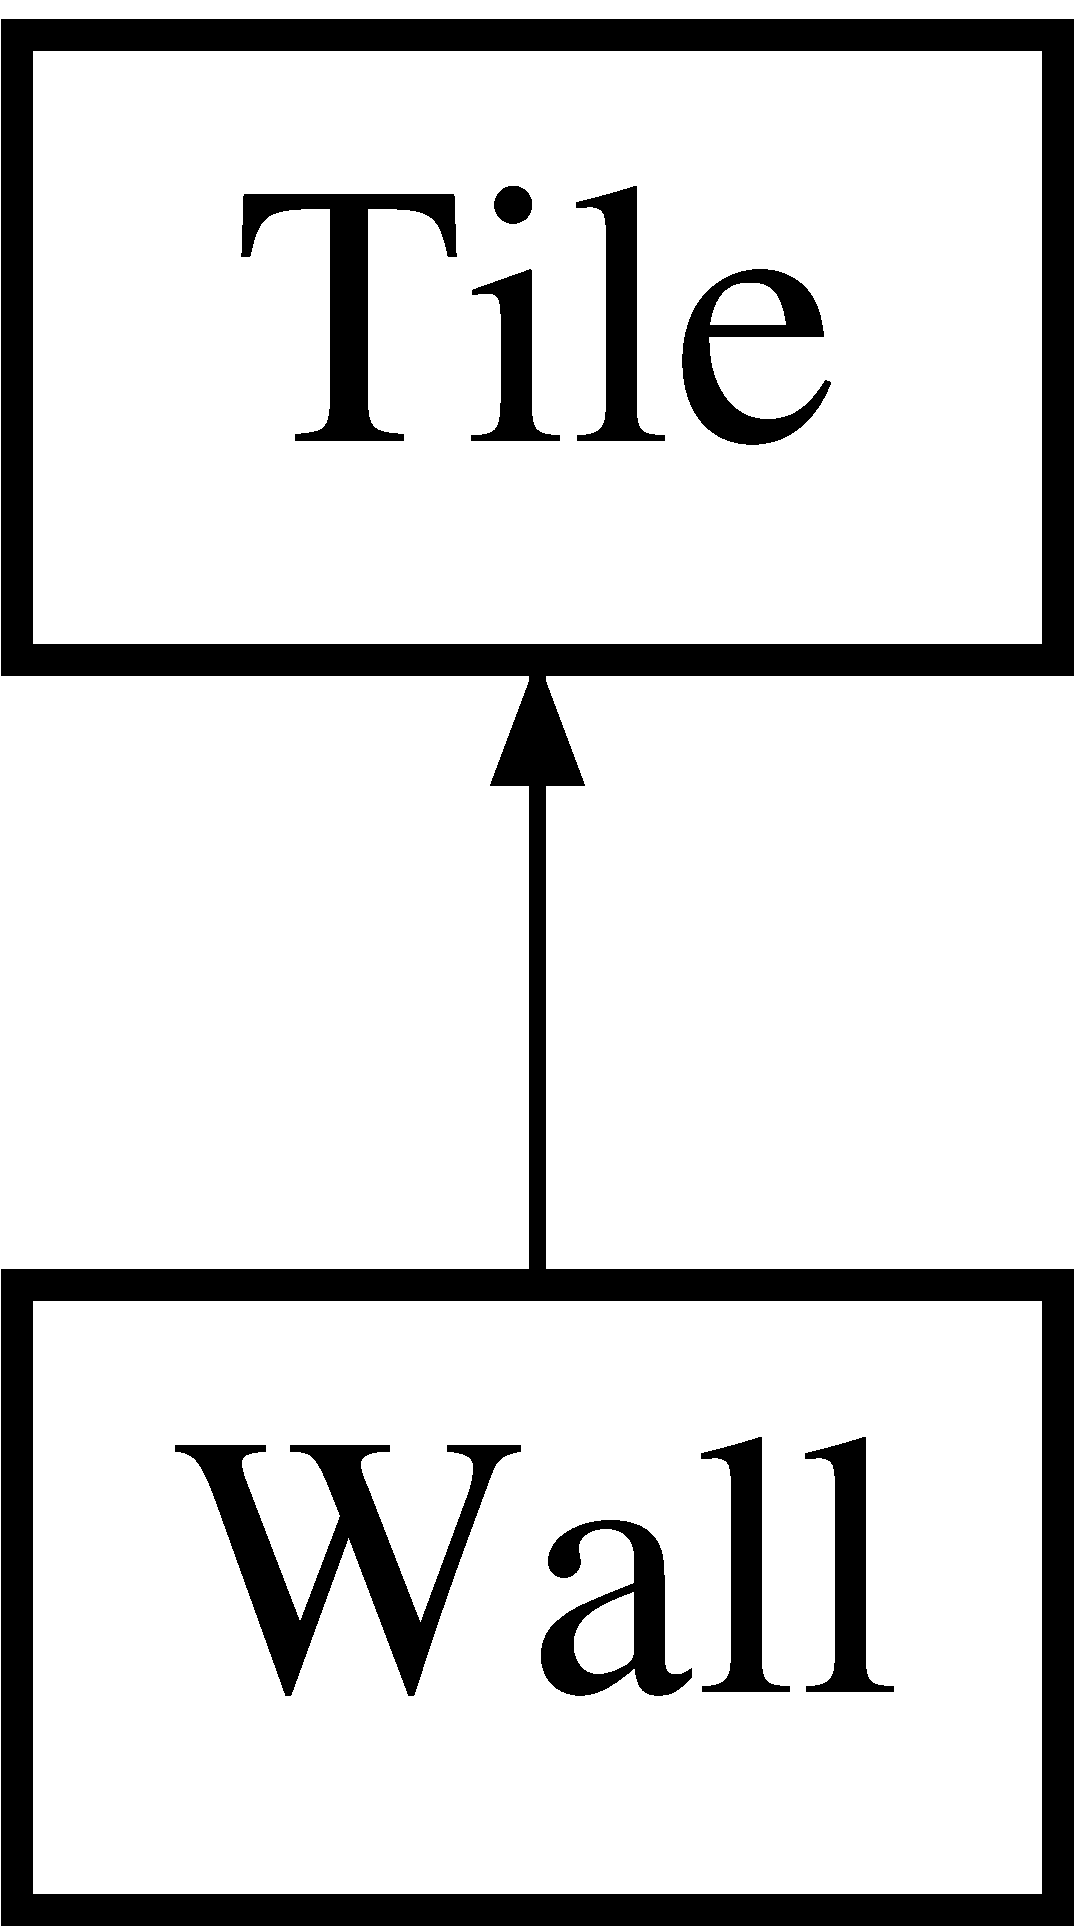
\includegraphics[height=2.000000cm]{class_wall}
\end{center}
\end{figure}
\subsection*{Public Member Functions}
\begin{DoxyCompactItemize}
\item 
\mbox{\Hypertarget{class_wall_aef304af86fdbcbee161df1d36db8bfd4}\label{class_wall_aef304af86fdbcbee161df1d36db8bfd4}} 
{\bfseries Wall} (sf\+::\+Vector2f pos)
\item 
\mbox{\Hypertarget{class_wall_a939a04ba33d30643467703820803e843}\label{class_wall_a939a04ba33d30643467703820803e843}} 
void {\bfseries load\+Image} ()
\end{DoxyCompactItemize}
\subsection*{Additional Inherited Members}


The documentation for this class was generated from the following files\+:\begin{DoxyCompactItemize}
\item 
Wall.\+h\item 
Wall.\+cpp\end{DoxyCompactItemize}

\hypertarget{class_worker}{}\section{Worker Class Reference}
\label{class_worker}\index{Worker@{Worker}}
\subsection*{Public Member Functions}
\begin{DoxyCompactItemize}
\item 
\mbox{\Hypertarget{class_worker_abcca1d98cfe682b3c80be626f97c2fb2}\label{class_worker_abcca1d98cfe682b3c80be626f97c2fb2}} 
{\bfseries Worker} (sf\+::\+Vector2f pos, \mbox{\hyperlink{class_node_layout}{Node\+Layout}} \&nodes, std\+::vector$<$ \mbox{\hyperlink{class_wall}{Wall}} $\ast$$>$ \&walls)
\item 
void \mbox{\hyperlink{class_worker_ad79617e69aff5ed4a22835f5e2b3cf7a}{update}} (float delta\+Time)
\item 
void \mbox{\hyperlink{class_worker_a18940af5e921feefc2373e120d66ff24}{render}} (sf\+::\+Render\+Window \&window)
\item 
void \mbox{\hyperlink{class_worker_a5d3aefa5dd3ad224ac861b4d69db95ed}{seek}} (float delta\+Time, sf\+::\+Vector2f v)
\item 
void \mbox{\hyperlink{class_worker_aa28cb0d23b4fc8e4a9480bab8d4724cf}{check\+Collisions}} (\mbox{\hyperlink{class_wall}{Wall}} $\ast$wall, float delta\+Time)
\item 
void \mbox{\hyperlink{class_worker_a1d02fa53eec27493717027977ffb6c54}{setup\+Path}} ()
\item 
void \mbox{\hyperlink{class_worker_a6f0cfcb460a9bc7fa3b2f1fa5ecc8b8a}{pick\+Random\+Dest}} (int random\+Index, int start\+Index)
\item 
void \mbox{\hyperlink{class_worker_ae9b32488617a0086772afd11529e3014}{normalise}} (sf\+::\+Vector2f \&v)
\item 
float \mbox{\hyperlink{class_worker_afaf8d6984011df1daa5ef9cd53abb4cc}{calculate\+Magnitude}} (sf\+::\+Vector2f v)
\item 
float \mbox{\hyperlink{class_worker_a00fc71b506eeeef4c431c40145057306}{calculate\+Magnitude}} (sf\+::\+Vector2f v1, sf\+::\+Vector2f v2)
\item 
\mbox{\Hypertarget{class_worker_a6bbf4cf7f718e3055f3fdc62a9482c58}\label{class_worker_a6bbf4cf7f718e3055f3fdc62a9482c58}} 
void {\bfseries set\+Rescued} (bool rescued)
\item 
\mbox{\Hypertarget{class_worker_afe18a64d13904bf62f2b27b21ff1fc67}\label{class_worker_afe18a64d13904bf62f2b27b21ff1fc67}} 
bool {\bfseries get\+Rescued} ()
\item 
\mbox{\Hypertarget{class_worker_a5e424fc42047b6b246f140c6c6190d29}\label{class_worker_a5e424fc42047b6b246f140c6c6190d29}} 
void {\bfseries set\+Abducted} (bool abducted)
\item 
\mbox{\Hypertarget{class_worker_acae6aa29c48a0da9b274cba3eb083319}\label{class_worker_acae6aa29c48a0da9b274cba3eb083319}} 
bool {\bfseries get\+Abducted} ()
\item 
\mbox{\Hypertarget{class_worker_ab4adcdb749d44a8be633466d2f20c9bd}\label{class_worker_ab4adcdb749d44a8be633466d2f20c9bd}} 
sf\+::\+Sprite {\bfseries get\+Sprite} ()
\item 
\mbox{\Hypertarget{class_worker_af8d4a69952c44caf94b37b75f42f343c}\label{class_worker_af8d4a69952c44caf94b37b75f42f343c}} 
sf\+::\+Vector2f {\bfseries get\+Pos} ()
\item 
\mbox{\Hypertarget{class_worker_a06c1679fcf49735590f36c4a84745ca1}\label{class_worker_a06c1679fcf49735590f36c4a84745ca1}} 
sf\+::\+Vector2f {\bfseries get\+Center} ()
\end{DoxyCompactItemize}


\subsection{Member Function Documentation}
\mbox{\Hypertarget{class_worker_afaf8d6984011df1daa5ef9cd53abb4cc}\label{class_worker_afaf8d6984011df1daa5ef9cd53abb4cc}} 
\index{Worker@{Worker}!calculate\+Magnitude@{calculate\+Magnitude}}
\index{calculate\+Magnitude@{calculate\+Magnitude}!Worker@{Worker}}
\subsubsection{\texorpdfstring{calculate\+Magnitude()}{calculateMagnitude()}\hspace{0.1cm}{\footnotesize\ttfamily [1/2]}}
{\footnotesize\ttfamily float Worker\+::calculate\+Magnitude (\begin{DoxyParamCaption}\item[{sf\+::\+Vector2f}]{v }\end{DoxyParamCaption})}

~\newline
... calc mag of a vector\mbox{\Hypertarget{class_worker_a00fc71b506eeeef4c431c40145057306}\label{class_worker_a00fc71b506eeeef4c431c40145057306}} 
\index{Worker@{Worker}!calculate\+Magnitude@{calculate\+Magnitude}}
\index{calculate\+Magnitude@{calculate\+Magnitude}!Worker@{Worker}}
\subsubsection{\texorpdfstring{calculate\+Magnitude()}{calculateMagnitude()}\hspace{0.1cm}{\footnotesize\ttfamily [2/2]}}
{\footnotesize\ttfamily float Worker\+::calculate\+Magnitude (\begin{DoxyParamCaption}\item[{sf\+::\+Vector2f}]{v1,  }\item[{sf\+::\+Vector2f}]{v2 }\end{DoxyParamCaption})}

... calc mag of two vectors\mbox{\Hypertarget{class_worker_aa28cb0d23b4fc8e4a9480bab8d4724cf}\label{class_worker_aa28cb0d23b4fc8e4a9480bab8d4724cf}} 
\index{Worker@{Worker}!check\+Collisions@{check\+Collisions}}
\index{check\+Collisions@{check\+Collisions}!Worker@{Worker}}
\subsubsection{\texorpdfstring{check\+Collisions()}{checkCollisions()}}
{\footnotesize\ttfamily void Worker\+::check\+Collisions (\begin{DoxyParamCaption}\item[{\mbox{\hyperlink{class_wall}{Wall}} $\ast$}]{wall,  }\item[{float}]{delta\+Time }\end{DoxyParamCaption})}

... collision between worker and wall\mbox{\Hypertarget{class_worker_ae9b32488617a0086772afd11529e3014}\label{class_worker_ae9b32488617a0086772afd11529e3014}} 
\index{Worker@{Worker}!normalise@{normalise}}
\index{normalise@{normalise}!Worker@{Worker}}
\subsubsection{\texorpdfstring{normalise()}{normalise()}}
{\footnotesize\ttfamily void Worker\+::normalise (\begin{DoxyParamCaption}\item[{sf\+::\+Vector2f \&}]{v }\end{DoxyParamCaption})}

~\newline
... normalise vector\mbox{\Hypertarget{class_worker_a6f0cfcb460a9bc7fa3b2f1fa5ecc8b8a}\label{class_worker_a6f0cfcb460a9bc7fa3b2f1fa5ecc8b8a}} 
\index{Worker@{Worker}!pick\+Random\+Dest@{pick\+Random\+Dest}}
\index{pick\+Random\+Dest@{pick\+Random\+Dest}!Worker@{Worker}}
\subsubsection{\texorpdfstring{pick\+Random\+Dest()}{pickRandomDest()}}
{\footnotesize\ttfamily void Worker\+::pick\+Random\+Dest (\begin{DoxyParamCaption}\item[{int}]{random\+Index,  }\item[{int}]{start\+Index }\end{DoxyParamCaption})}

~\newline
... selects random destination for worker\mbox{\Hypertarget{class_worker_a18940af5e921feefc2373e120d66ff24}\label{class_worker_a18940af5e921feefc2373e120d66ff24}} 
\index{Worker@{Worker}!render@{render}}
\index{render@{render}!Worker@{Worker}}
\subsubsection{\texorpdfstring{render()}{render()}}
{\footnotesize\ttfamily void Worker\+::render (\begin{DoxyParamCaption}\item[{sf\+::\+Render\+Window \&}]{window }\end{DoxyParamCaption})}

~\newline
... renders the worker in the game world\mbox{\Hypertarget{class_worker_a5d3aefa5dd3ad224ac861b4d69db95ed}\label{class_worker_a5d3aefa5dd3ad224ac861b4d69db95ed}} 
\index{Worker@{Worker}!seek@{seek}}
\index{seek@{seek}!Worker@{Worker}}
\subsubsection{\texorpdfstring{seek()}{seek()}}
{\footnotesize\ttfamily void Worker\+::seek (\begin{DoxyParamCaption}\item[{float}]{delta\+Time,  }\item[{sf\+::\+Vector2f}]{v }\end{DoxyParamCaption})}

~\newline
... seeks to target\mbox{\Hypertarget{class_worker_a1d02fa53eec27493717027977ffb6c54}\label{class_worker_a1d02fa53eec27493717027977ffb6c54}} 
\index{Worker@{Worker}!setup\+Path@{setup\+Path}}
\index{setup\+Path@{setup\+Path}!Worker@{Worker}}
\subsubsection{\texorpdfstring{setup\+Path()}{setupPath()}}
{\footnotesize\ttfamily void Worker\+::setup\+Path (\begin{DoxyParamCaption}{ }\end{DoxyParamCaption})}

... generates random path for worker\mbox{\Hypertarget{class_worker_ad79617e69aff5ed4a22835f5e2b3cf7a}\label{class_worker_ad79617e69aff5ed4a22835f5e2b3cf7a}} 
\index{Worker@{Worker}!update@{update}}
\index{update@{update}!Worker@{Worker}}
\subsubsection{\texorpdfstring{update()}{update()}}
{\footnotesize\ttfamily void Worker\+::update (\begin{DoxyParamCaption}\item[{float}]{delta\+Time }\end{DoxyParamCaption})}

~\newline
... updates workers who havent been abducted or rescued

The documentation for this class was generated from the following files\+:\begin{DoxyCompactItemize}
\item 
Worker.\+h\item 
Worker.\+cpp\end{DoxyCompactItemize}

\hypertarget{class_world}{}\section{World Class Reference}
\label{class_world}\index{World@{World}}
\subsection*{Public Member Functions}
\begin{DoxyCompactItemize}
\item 
\mbox{\Hypertarget{class_world_a6be69ff54f7f29713c0954cabe34aecc}\label{class_world_a6be69ff54f7f29713c0954cabe34aecc}} 
void {\bfseries render} (sf\+::\+Render\+Window \&window)
\item 
\mbox{\Hypertarget{class_world_a0150607a49c2400d5c848159dd02d533}\label{class_world_a0150607a49c2400d5c848159dd02d533}} 
void {\bfseries init} ()
\item 
\mbox{\Hypertarget{class_world_a6f861499defce9ddb7f660e4c7f4a194}\label{class_world_a6f861499defce9ddb7f660e4c7f4a194}} 
void {\bfseries update} (float delta\+Time)
\end{DoxyCompactItemize}
\subsection*{Public Attributes}
\begin{DoxyCompactItemize}
\item 
\mbox{\Hypertarget{class_world_a15cab1c818f25a605c8379983618a5fe}\label{class_world_a15cab1c818f25a605c8379983618a5fe}} 
sf\+::\+View {\bfseries m\+\_\+radar}
\item 
\mbox{\Hypertarget{class_world_addf54f12f3a1e9c8f120265bafa3474e}\label{class_world_addf54f12f3a1e9c8f120265bafa3474e}} 
\mbox{\hyperlink{class_player}{Player}} $\ast$ {\bfseries player}
\item 
\mbox{\Hypertarget{class_world_a7ad719bc4a4c234d4610a9657f1ecb30}\label{class_world_a7ad719bc4a4c234d4610a9657f1ecb30}} 
\mbox{\hyperlink{class_space_station}{Space\+Station}} {\bfseries m\+\_\+space\+Station}
\item 
\mbox{\Hypertarget{class_world_a666d6636240895d601d85f4ca15df01b}\label{class_world_a666d6636240895d601d85f4ca15df01b}} 
\mbox{\hyperlink{class_nest}{Nest}} $\ast$ {\bfseries m\+\_\+nest}
\item 
\mbox{\Hypertarget{class_world_ad87050cff8d746edba3b7be07a9b764e}\label{class_world_ad87050cff8d746edba3b7be07a9b764e}} 
\mbox{\hyperlink{class_nest}{Nest}} $\ast$ {\bfseries m\+\_\+nest2}
\item 
\mbox{\Hypertarget{class_world_a2d978612cb7f10e3b66f89e0fcfa9c6a}\label{class_world_a2d978612cb7f10e3b66f89e0fcfa9c6a}} 
\mbox{\hyperlink{class_nest}{Nest}} $\ast$ {\bfseries m\+\_\+nest3}
\item 
\mbox{\Hypertarget{class_world_a0f09ef171e221568a0428ef3fdefbbb2}\label{class_world_a0f09ef171e221568a0428ef3fdefbbb2}} 
\mbox{\hyperlink{class_a_star}{A\+Star}} $\ast$ {\bfseries a\+Star}
\end{DoxyCompactItemize}


The documentation for this class was generated from the following files\+:\begin{DoxyCompactItemize}
\item 
World.\+h\item 
World.\+cpp\end{DoxyCompactItemize}

%--- End generated contents ---

% Index
\backmatter
\newpage
\phantomsection
\clearemptydoublepage
\addcontentsline{toc}{chapter}{Index}
\printindex

\end{document}
